\documentclass[draft]{agujournal2019}
\usepackage{url} %this package should fix any errors with URLs in refs.
\usepackage{lineno}
\usepackage{amsmath}
\usepackage{sidecap}
\usepackage[inline]{trackchanges} %for better track changes. finalnew option will compile document with changes incorporated.
\usepackage{soul}
\linenumbers

\draftfalse

\journalname{Tectonics}


\begin{document}

\title{Laurentia's continued motion into the Neoproterozoic: new paleomagnetic constraint from the Jacobsville Formation}

\authors{Yiming Zhang\textsuperscript{1}, Blake Hodgin\textsuperscript{1}, Nicholas Swanson-Hysell\textsuperscript{1}, James Pierce\textsuperscript{1}, Anthony Fuentes\textsuperscript{1}}

\affiliation{1}{Department of Earth and Planetary Science, University of California, Berkeley, CA, USA}

\correspondingauthor{Yiming Zhang}{yimingzhang@berkeley.edu}

\begin{keypoints}
\item A new paleomagnetic pole from the ca. 992 Ma Jacobsville Formation 
\item Reversals put younger bounds on the normal Keweenawan superchron 
\item The new pole indicates the Grenville Loop could be younger than thought
\end{keypoints}


\begin{abstract}
The ca. 1.1 Ga North American Midcontinent Rift resulted in protracted magmatism and associated deposition of sediments during rift-related extension and post-rift thermal subsidence. Coeval with the cessation of rifting and a decrease of Laurentia's plate speed is the onset of the ca. 1090-980 Ma Grenvillian Orogeny along the eastern margin. The far-field stress of the orogeny is interpreted to have propagated into the interior of Laurentia and inverted the Midcontinent Rift, deforming the post-rift Jacobsville Formation whose maximum depositional age has been constrained to be ca. 992 Ma. We develop a new paleomagnetic pole from red beds of the Jacobsville Formation along five stratigraphic sections in northern Michigan, USA. High-resolution thermal demagnetization experiments resolve detrital magnetic remanence that pass a fold test and two conglomerate tests. Our results confirm the occurrence of geomagnetic field reversals during the deposition of Jacobsville Formation, providing constraints for the maximum duration of the Keweenawan superchron. An inclination corrected paleomagnetic pole position from the Jacobsville Formation confirm continued plate motion of Laurentia across the equator in the late Mesoproterozoic to early Neoproterozoic. The new pole from the interior of Laurentia indicates the paleomagnetic poles developed from the Grenville Province most likely record coherent plate motion after major continental collision during the development of the supercontinent Rodinia.
% rather than recording a significant crustal shortening.
\end{abstract}

% \section*{Plain Language Summary}
% [ enter your Plain Language Summary here or delete this section]


\section*{Keywords}
Neoproterozoic\\
Laurentia  \\
Paleogeography\\
\

apparent polar wander path\\
Inclination shallowing\\
Grenville\\
Keweenawan superchron\\
Red bed\\

\section*{Introduction}

The extensively studied paleomagnetic records of the ca. 1109 Ma to 1084 Ma North American Midcontinent Rift (i.e. the Keweenawan Track) provide crucial constraints on global paleogeography in the Mesoproterozoic \cite{Swanson-Hysell2019a}. As a result, the Keweenawan Track has become a central record for reconstructing the development of the ancient supercontinent Rodinia \cite{2021a}. As the rifting ceased and subsequently inverted following the onset of the Grenvillian Orogeny on Laurentia's eastern margin (Fig. \ref{fig:Geologic_map}), magmatism in the interior of Laurentia entered a period of quiescence that could have lasted for as long as $\sim$300 Myr until the emplacement of the ca. 780 Ma Gunbarrel large igneous province \cite{Harlan2003a, Mackinder2019a}. Due to this magmatic gap, Laurentia and its conjugate continents' paleogeographic configuration in the late Mesoproterozoic to mid-Neoproterozoic has remained largely uncertain \cite{Swanson-Hysell2021c}.

\begin{figure*}[h!]
\centering
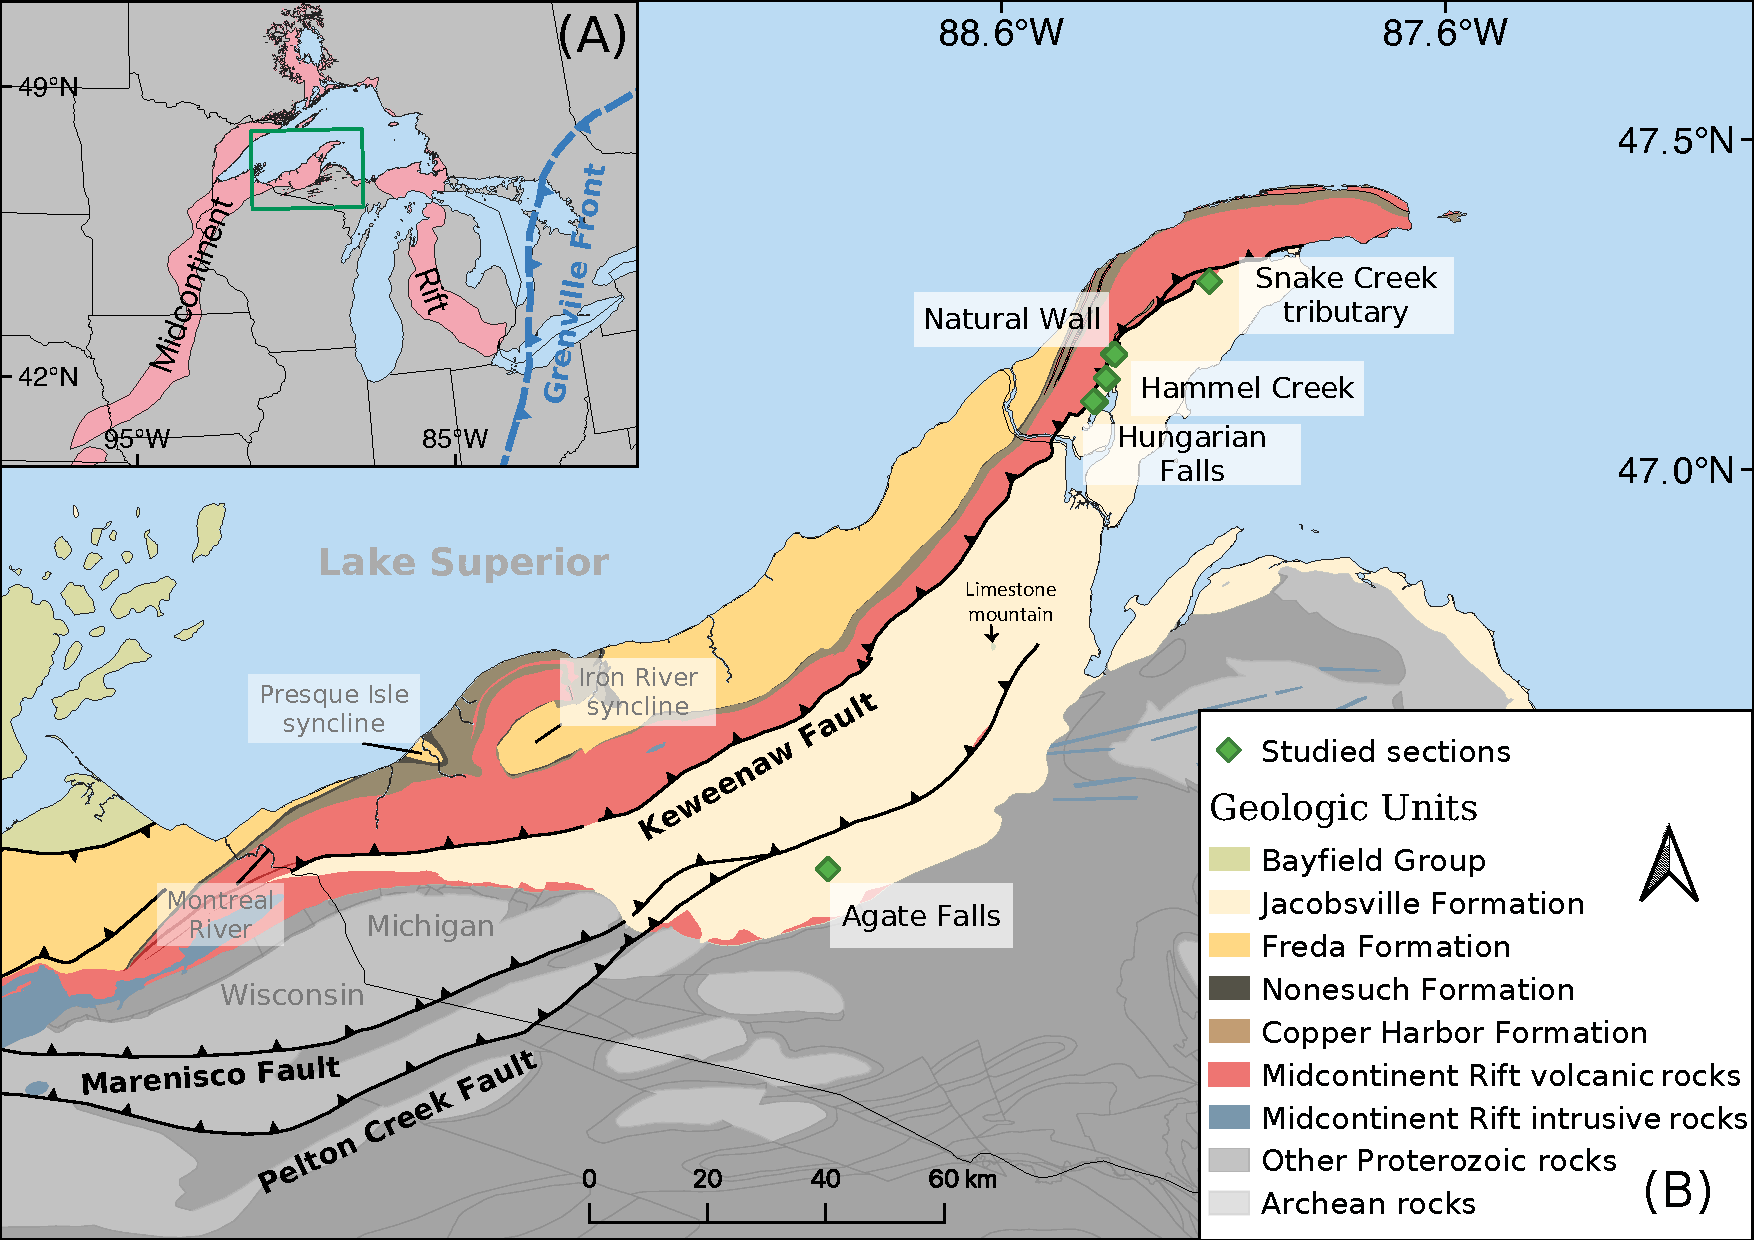
\includegraphics[width=\textwidth]{Geologic_map.pdf}
\caption{(A) Regional map showing location of the Grenville Front relative to the study area. The inset green box shows the extent of panel B. (B) Geologic map of northern Michigan and Wisconsin showing Midcontinent Rift igneous and sedimentary rocks, the Jacobsville Formation, other older Proterozoic rocks, and major post-rift thrust faults. Jacobsville stratigraphic sections along which paleomagnetic samples were collected in this study are shown as green diamond symbols.}
\label{fig:Geologic_map}
\end{figure*}

When igneous rock records are lacking, paleomagnetic data recorded by sedimentary rocks (e.g. red beds) can provide useful insights into the ancient geomagnetic field and record paleogeographic positions of sedimentary basins. In the Midcontinent Rift, the paleomagnetic poles developed from the ca. 1075 Ma Nonesuch Formation and the ca. 1070 Ma upper Freda Formation of the Oronto Group sediments that overlie the Midcontinent Rift volcanics in southern Lake Superior area (Fig. \ref{fig:Geologic_map}) provide crucial constraints for Laurentia's latitude, orientation, and plate motion in the late Mesoproterozoic \cite{Henry1977a, Swanson-Hysell2019a, Swanson-Hysell2019b}. 

On top of the Oronto Group sediments overlies the post-rift Jacobsville Formation which was partly deformed during the inversion of the Midcontinent Rift (Fig. \ref{fig:Geologic_map}; \citeA{Hamblin1958a, Hodgin2022a, DeGraff2022a}). The Jacobsville Formation also contains abundant red beds which offer the opportunity to further extend the reconstruction of the apparent polar wander path of Laurentia toward more recent times \cite{Hamblin1958a, Roy1978a}. U-Pb detrital zircon ages and U-Pb calcite ages from late-kinematic veins constrain the maximum depositional age of the Jacobsville Formation to be ca. 992 Ma \cite{Hodgin2022a}. Developing paleomagnetic data from the Jacobsville Formation will allow further development of Laurentia's paleogeographic evolution in the late Mesoproterozoic to early Neoproterozoic. 

Challenges exist in interpreting sedimentary paleomagnetic records. Primary detrital remanence acquired during settling of magnetic particles in the water column can be masked as secondary magnetic minerals (e.g. pigmentary hematite) that precipitate and grow within pore spaces of host sedimentary rocks syn- to post-deposition. In red beds, it has been found that formation of the pigmentary hematite can significantly post-date the timing of sediment deposition, resulting in the chemical remanent magnetization being secondary, superimposed upon the primary remanent magnetization carried by detrital grains \cite{Butler1992a}. To isolate the remanence components of the red beds of the Jacobsville Formation, \citeA{Roy1974a, Roy1978a} adopted a method first applied by \citeA{Collinson1965c} to preferentially remove fine-grained pigmentary hematite through prolonged immersion in concentrated HCl acid whereas leaving the coarser detrital grains that are more resistant to dissolution in place. Studies applying paired acid etching demagnetization and thermal demagnetization show that the pigmentary hematite grains tend to have lower unblocking temperatures than detrital ones \cite{Tauxe1980a, Bilardello2010c}. High-resolution thermal demagnetization experiments with temperature intervals as small as 1-2 \textdegree C have shown to be effective in isolating detrital remanence from chemical remanence as coarser hematite grains tend to have higher unblocking temperatures \cite{Swanson-Hysell2019b}. In particular, a conglomerate test on a suite of fluvial intraclasts of the red beds in the Freda Formation shows that via thermal demagnetization one can isolate detrital magnetization vectors (which are reoriented in random directions in the clasts) from the secondary components carried by co-occurring authigenic hematite (which yield similar directions amongst clasts) \cite{Swanson-Hysell2019b}. 

Paleomagnetism of red beds has also been challenged by the controversial issue of correcting for inclination shallowing \cite{King1955a, Tauxe2004b, Bilardello2016b}, which is necessary due to the rotation of detrital magnetic grains to be parallel to bedding caused by authigenic processes such as compaction during lithification. As a result, inclinations recorded by sediments often have shallower angles than the local field inclinations during the time of deposition. To estimate the amount of inclination shallowing in a given package of sedimentary rocks, \citeA{Tauxe2004b} developed a statistical model (i.e. the elongation/inclination method) that evaluates the deviation of the distribution of a large number ($>$100) of observed sedimentary paleomagnetic directional data with the predicted distribution given by a paleosecular variation model developed for the past 5 Myr (TK03) under the the geocentric axial dipole (GAD) hypothesis. Although the TK03 paleosecular variation model is based on data of relatively recent geomagnetic field, it has been shown to be compatible with data from the ca. 1.1 Ga lava flows of the Midcontinent Rift \cite{Tauxe2009a}. Further, \citeA{Pierce2022a} showed that the E/I method passes a field test for the 1.1 Ga Cut Face Creek Sandstone as the method successfully corrects the shallow paleomagnetic inclination of the sediments to that of the lava flows that bracket them. That study also further extended the method to better represent uncertainties associated with the amount of inclination shallowing when reporting sedimentary paleomagnetic pole positions by using the spherical elliptical Kent distribution \cite{Kent1982a} instead of the circular Fisher distribution \cite{Fisher1953a}. 

In this study, we investigate the hematite-bearing, fine-grained sandstone to siltstone lithofacies along five stratigraphic sections of the Jacobsville Formation. High-resolution thermal demagnetization data on siltstone intraclasts that were eroded by fluvial processes and redeposited at two locations constrain the timing of hematite acquisition by revealing a primary component that formed prior to the erosion of the clasts within the depositional environment and a secondary component that formed following their redeposition. We then use a paleomagnetic fold test to further constrain the timing of detrital remanence acquisition in association with the structural inversion of the Midcontinent Rift. Finally, we develop a new inclination-corrected paleomagnetic pole for the Jacobsville Formation based on a large number of samples and investigate the paleo-continental configuration of Laurentia and its association with the development of the supercontinent Rodinia. 


% The end of the ca. 1109 Ma to 1084 Ma intracontinental Midcontinent Rift magmatism and extension was marked by a transition to deposition of sedimentary rocks of the Oronto Group \cite{Ojakangas2001a} as the rift basin thermally subsided prior to the rift undergoing contractional deformation in the later stages of the Grenvillian orogeny \cite{Cannon1992b, Hodgin2022a}.

%  that has become central to the reconstruction of paleogeography of the assembly of supercontinent Rodinia. In addition to syn-rift rocks preservation, the cessation and later inversion of the rift allowed the development of syn-to post-rift basin development which accommodated the deposition of the ca. 1080 - 1050 Ma Oronto Group sedimentary rocks that are in total about 5 km thick. Overlying the Oronto Group is the Jacobsville formation which has been interpreted to be deposited in a back-bulge setting associated with the far-field propagation of the crustal-scale deformation caused by the Grenvillian Orogeny.



% A leading tectonic model for the cessation of the Midcontinent Rift and extension is that it occurred due to far-field compressional stress associated with the ca. 1090-980 Ma Grenvillian orogeny \cite{Cannon1992a}, when the collision of Laurentia with its conjugate margins led to the development of a back-bulge basin, accommodating the deposition of the Jacobsville Formation sediments as the inversion of the Midcontinent Rift progressed. Recent re-examination of the maximum deposition age of the Jacobsville Formation using zircon U-Pb whole grain chemical abrasion isotope dilution thermal ionization mass spectrometry has updated the maximum deposition age of the Jacobsville Formation to be ca. 990 Ma \cite{Hodgin2022a}. Such age constraint is consistent with backbulge subsidence model \cite{DeCelles, 2012}, indicating that the Jacobsville Formation may have been deposited in a Grenvillian foreland basin system that resulted from lithospheric flexure induced by orogenic loading \cite{Rivers2012a}. The relatively young age of the Jacobsville Formation compared to other Midcontinent Rift rocks makes the Jacobsville Formation an crucial target for further reconstructing the global paleogeography in the late Proterozoic. For further refining the paleogeographic connection between the poles of the Grenville Loop and those of the Keweenawan Track. 



% Paleomagnetic data for the Jacobsville Formation have led to a paleomagnetic pole position that appears to be a continuation of the Keweenawan Track from the Oronto Group poles (Roy and Robertson, 1978; Fig. 7; Table 4). As a result, its age has been interpolated to be latest Mesoproterozoic (e.g., 1020 Ma in Li et al., 2008) such that it was deposited prior to the ca. 1000 Ma Grenville loop poles. However, this age assignment has recently been questioned on the basis of laser-ablation–inductively cou- pled plasma–mass spectrometry (LA-ICP-MS) U-Pb detrital zircon dates from Jacobsville Sandstone samples. Malone et al. (2016) interpreted a maximum depositional age of 959 ± 19 Ma based on the weighted mean of the four youngest grains from 2050 LA-ICP-MS zircon dates. A similar age was proposed on the basis of the youngest LA-ICP-MS U-Pb dates in the study of Craddock et al. (2013). This young maximum interpreted age is intriguing because it suggests the unconformity above the Freda Sandstone spans at least 100 m.y. and was followed by continued sedimentation in the region long after rift activity. Nevertheless, the paleo- magnetic pole of the Jacobsville Sandstone (Roy and Robertson, 1978) appears to extend the Keweenawan Track from the Oronto Group poles in a manner that may be more consistent with deposition of the Jacobsville Formation in the late Mesoproterozoic. Given the conflict with this inferred age, the large uncertainty of individual LA-ICP-MS dates, and the possibility of outlier dates in such a large data set, it is beneficial to interpret the age of the youngest Jacobsville zircons dated CA-ID-TIMS to obtain more precise constraints. Using CA-ID-TIMS, a recent study by Hodgin et al (2022) redefines the maximum deposition age of the Jacobsville Formation as ca. 993 Ma.



% The extensive paleomagnetic studies of the well-preserved late Mesoproterozoic to Neoproterozoic rocks of North America have provided the central record for global paleogeography reconstruction during the assembly and rearrangement of the postulated supercontinent Rodinia. Paleomagnetic studies of rocks from Laurentia have led to a series of paleomagnetic poles that form an apparent polar wander path (APWP) known as the ``Logan Loop" for the older high latitude poles at its apex that continues into the ``Keweenawan Track" of younger lower latitude poles that form a progression as the APWP heads toward the ``Grenville Loop" \citep{Swanson-Hysell2019a}. In particular, recent advances in pairing high-precision zircon U-Pb geochronology with high-quality paleomagnetic poles significantly improved the resolution of the Keweenawan Track and revealed Laurentia's rapid motion ($>$20 cm/yr) during the Midcontinent Rift magmatic activity from ca. 1110 Ma to ca. 1085 Ma \citep{Swanson-Hysell2019a}. 

% As the Midcontinent Rift magmatic activity wanes its strength and evolved into a failed intracontinental rift, Laurentia experienced a long period of magmatic quiescence in its interior, where basin subsidence dominated the rift basin. This was followed by the Grenville Orogeny, causing the the inversion of the rift along thrust belts such as the Keweenaw Fault (Fig. xxx). The lack of extensive magmatism from ca.1080 Ma to ca. 980 Ma in the Laurentia interior resulted in a significant gap (for at least 50 myr) of paleomagnetic poles between the Keweenawan Track (developed from interior Laurentia igneous and sedimentary rocks) and the Grenville Loop (poles developed from the Grenville Province rocks) (Fig. xxx; \cite{Swanson-Hysell2019a}).  

% Due to the lack of pmag records from the interior Laurentia, various hypotheses for the spatial relationship between the end of the Keweenawan Track and the Grenville Loop have been debated. One model argues for that the difference in pole locations indicates that the Grenville Province was once thousands of kilometers away from Interior Laurentia and was progressively approaching the southern margin of Laurentia in the late Mesoproterozoic \citep{Halls2015}. A corollary of this hypothesis is that there had to be a 4000 km shortening during the Grenville orogeny - colliding Amazonia-Laurentia. The other model favors that the Grenville Loop is a continuation of the Keweenawan Track - that the southerly continental drift of Laurentia continued across the equator onto the southern hemisphere from ca. 1070 Ma to ca.1000 Ma. and  approached this problem by developing data from metamorphosed dike and anorthosite and argued for Grenville  

% Paleomagnetic poles from the interior of Laurentia during the quiescence magmatism period is thus crucial for reconcile the discordant paleomagnetic poles of the Keweenawan Track and the Grenville Loop. The
% %Q: what are you using the poles from rocks that we know are from the Laurentia interior? (outside of the Grenville package?)

% This new age constraint on the Jacobsville provides crucial insight into the tectonic evolution of the Midcontinent Rift and the inversion of the extensional region into a compressional region due to the Grenville orogen. It also makes the Jacobsville sandstone a unique opportunity to investigate Laurentia's paleogeographical position at ca. 1 Ga as a long period of magmatic quiescence for $\sim$50 myr precedes Jacobsville deposition left a gap in Laurentia apparent polar wander path between the Keweenawan Track and the Grenville Loop (Fig. xxx). 

% Jacobsville sedimentation was preceded by a long period of volcanic and tectonic quiescence and cratonic stability so that bedrock surfaces became blanketed by paleosol and a surface of chemically resistant debris was dominated by quartz and iron-formation. 

% Previous paleomagnetic study on the red beds within the Jacobsville by \cite{Roy1978a} observed different components using AF, thermal, and chemical demagnetizations. Recognized dual polarities and recognized the complex remanence acquisition of red beds which lead to three isolated remanence components from the Jacobsville. However, that study did not recognize the problem of inclination shallowing and did not apply correction factor on the results. Moreover, the course demagnetization steps during thermal demagnetization would have had limited resolution for distinguishing the depositional remanent magnetization (DRM) and secondary chemical remanent magnetization (CRM) which have recently been shown to unblock over a narrow temperature window \cite{Swanson-Hysell2019b}. 


\section*{Geologic settings}

\subsection*{Structure}
The ca. 1109 Ma to 1084 Ma North American Midcontinent Rift is a major intracontinental rift system that extends over 2000 km through the Laurentia craton (Fig. \ref{fig:Geologic_map}). However, the rifting failed to separate Laurentia into two continents. As its magmatism waned and thermal subsidence progressed in the rift basin, the $>$4 km of ca. 1085-1050 Ma Oronto Group sediments \cite{Fairchild2017a, Swanson-Hysell2019a} were deposited conformably on top of the rift volcanics (Fig. \ref{fig:Geologic_map}; \citeA{Cannon1992a}). Subsequently, the rift was inverted as the ca. 1090-980 Ma Grenvillian Orogeny commenced on the eastern margin of Laurentia (Fig. \ref{fig:Geologic_map}), eventually resulting in the propagation of far-field compressional stress deep into the interior of Laurentia \cite{Cannon1993a, Cannon1994a}. 

During the inversion, Paleoproterozoic and Archean crust was uplifted via thrust faults such as the Marenisco fault and the Pelton Creek fault, forming the crustal-scale Montreal River monocline (Fig. \ref{fig:Geologic_map}; \citeA{Cannon1993a}). The southern part of the post-rift Jacobsville Formation overlies an erosional angular unconformity that developed on lithologies that were exhumed through this earlier reverse motion (Fig. \ref{fig:Geologic_map}; \citeA{Hamblin1958a, Cannon1993a, Kalliokoski1982a}). More recent mapping of the Jacobsville Formation has also found that it can sometimes onlap the Midcontinent Rift volcanics within or adjacent to the Keweenaw Fault system around Bete Grise Bay on the Keweenaw Peninsula (Fig. \ref{fig:Geologic_map}; \citeA{Tyrrell2019a, Mueller2021a}). Field observations find erosional contact and development of paleosol between the Jacobsville Formation and underlying volcanic rocks \cite{Hamblin1958a, Kalliokoski1975a}, and interpretations of seismic reflection data show that sedimentary rocks interpreted to be Jacobsville Sandstone lie unconformably on the Oronto Group \cite{Cannon1989a}. These observations are consistent with the interpretation that there was a prolonged period of sedimentation quiescence and net erosion between the end of Oronto Group deposition and onset of Jacobsville Formation deposition. Based on dates from Cannon et al 1993 (and deformation of the Freda Fm within the Montreal River monocline) paired with new dates on the Jacobsville Fm (Hodgin et al., 2022), this time period of quiescence may have lasted up to ~60 Myrs from ca. 1050 until ca. 990 Ma. The overall extent of the Jacobsville Formation has been mapped along the lake shore of the Keweenaw Peninsula from northern Michigan, USA, to the north side of Michipicoten Island and perhaps to northern Sault Ste Marie, Canada (Fig. \ref{fig:Geologic_map}; \citeA{Hamblin1958a}). 

As far-field stresses from the Grenvillian Orogeny propagated into the interior of Laurentia, the previously thinned crust of the Midcontinent Rift was structurally inverted by crustal-scale thrusts, such as the Keweenaw Fault which extends $\sim$250km from ...refs here. Final inversion of the Keweenaw Fault during the Grenvillian Orogeny thrust Midcontinent Rift volcanics over the Jacobsville strata, which were folded in the footwall of the fault.  along much of the Keweenaw fault which extends $\sim$250 km from the tip of the Keweenaw Peninsula in northern Michigan southeastward to a termination in northeastern Wisconsin (Fig. \ref{fig:Geologic_map}; \citeA{Cannon1996a, Cannon2001a, DeGraff2022a}). Syndepositional faulting that took place during Jacobsville deposition is inferred from ... rift volcanic clasts where eroded into the Jacobsville basin at the same time when sediments from the older basement rocks along with distal input from the Grenville Province were deposited within the Jacobsville back-bulge basin system that in general wedges toward the northwest (Fig. \ref{fig:Geologic_map}; \cite{Hedgman2014a, Hodgin2022a}. Next to the footwall of the Keweenaw fault, folding has also been recorded by strata of the upper Jacobsville Formation in contact with the volcanics \cite{Cannon1993a}. One famous remnant of that late-stage deformation is the Natural Wall ravine where sub-vertical sandstone beds are preserved (Fig. \ref{fig:Geologic_map}; \cite{Hamblin1958a}). On the shore of Bete Grise Bay near the northeastern end of Keweenaw Peninsula, the Keweenaw fault is interpreted to have accommodated Grenville compressional stresses by forming a series of segmented en echelon thrusts \cite{Tyrrell2019a}. The timing of such faulting could be coeval with the deposition of the upper Jacobsville Formation, leading to the nonconformable onlapping of the Jacobsville sediments over the volcanics in addition to the thrust faulting relationship between the two units. Ca. 985 Ma late-kinematic calcite that precipitated within the hanging wall of the Keweenaw Fault and ca. 992 Ma maximum deposition age from detrital zircons of the Jacobsville Formation in the footwall constrain the timing of the final inversion of the Keweenaw Fault to be during the Rigolet phase of the Grenvillian Orogeny \cite{Hodgin2022a}. 

\subsection{Sedimentology and general stratigraphy}

% It has been interpreted that the Jacobsville Sandstone is equivalent to the Bayfield Group in northern Wisconsin, and the Fond Du Lac and Hinckley formations in Minnesota. Their shared lithofacies of basal conglomerate, cross-bedded fluvial fine to medium grained sandstone, and interbedded red micaceous siltstone could support the interpretation that these sedimentary rocks formed during a common period of post-rift basin formation following rift-related magmatism of the Midcontinent Rift. 
\begin{figure*}[h!]
\centering
\includegraphics[width=0.9\textwidth]{Field_photo.png}
\caption{\scriptsize Field photos of red beds of the Jacobsville Formation sampled in this study. At Baby Snake Creek and the Natural Wall ravine in northern Keweenaw Peninsula, intervals of red fine-grained sandstone beds can be found through the steeply dipping to overturned basal strata near the Keweenaw Fault (A,C) and also the nearly horizontal top strata (B,D). At Hungarian Falls, relatively thick intervals of fine-grained red sandstone to siltstone beds separated by hematite-depleted arenite to arkosic sandstones or conglomerates are found along a $\sim$100-meter-tall waterfall (E). Abundant reoriented siltstone rip-up clasts often exist within the conglomeratic layers above siltstone beds (F). Drill cores or block samples of these rip-up clasts are sampled for the paleomagnetic conglomerate test presented in Fig. \ref{fig:Intraclast_pmag}. At Agate Falls, nearly flat-lying red fissile shale beds are exposed due to waterfall incision (G). Subrounded detrital mica grains deposited parallel to the bedding plane are often associated with the siltstone facies. Another set of siltstone rip-up clasts were sampled from a conglomeratic layer near the basal exposure for the paleomagnetic conglomerate test. }
\label{fig:Field_photo}
\end{figure*}

The Jacobsville Formation is a fluvial sequence of feldspathic and quartzose conglomerates, sandstones, siltstones, and shales completely devoid of lava flows or cross-cutting igneous dikes although cross-cutting clastic dikes have been observed. Abundant near the bottom section in the southern exposures of the Jacobsville Formation, conglomerate facies typically have provenance sourced from Paleoproterozoic lithologies such as vein quartz and iron formation clasts \cite{Hamblin1958a, Kalliokoski1982a}. The occurrence of these conglomerates in proximity to the Keweenaw, Marenisco, and Pelton Creek thrust faults is interpreted to represent syn-depositional development of local relief \cite{Kalliokoski1982a, Hedgman2014a}). It is in general more quartz-rich than the Oronto Group sediments \cite{Hamblin1958a}. 

Close to the Keweenaw Fault in central Keweenaw Peninsula (Fig. \ref{fig:Geologic_map}), the Jacobsville Formation consists dominantly of quartz-rich, cross-bedded, medium-grained sandstone, with locally abundant clast-supported pebble to cobble conglomerate, and interbeds of red, hematite-bearing, micaceous shaly siltstone to fine-grained sandstone (Hungarian Falls, Hammel Creek, Natural Wall; Fig. \ref{fig:strat_column}). In this region, the conglomerate contains abundant volcanic clasts likely derived from uplifted Midcontinent Rift volcanics \cite{Irving1885a, Brojanigo1984a}. This clast-supported lithofacies can include siltstone rip-up clasts or channelized lenses of siltstones. Occurrence of red siltstone to sandstone beds are also commonly interbedded with sandstone and conglomerate \cite<e.g.>{Hamblin1958a, Irving1885a}. They typically appear brick-red to dark-red, consisting of find-grained arenite to arkosic sandstone and siltstone sometimes with minor grey reduction spots (Fig. \ref{fig:Field_photo}). Rounded detrital mica grains up to $\sim$5mm in size can be found commonly within very fine, fissile siltstone and shaly strata (Fig. \ref{fig:Field_photo}). 

The exact stratigraphic association between sections of the Jacobsville Formation in the central Keweenaw Peninsula and those exposed at Agate Falls and Baby Snake Creek is difficult to constrain as the thickness of the Jacobsville strata can vary significantly through the peninsula \cite{Hamblin1958a, Kalliokoski1982a} and are not fully exposed at or in between the studied localities. As a result, various interpretations could exist for the relative stratigraphy at different localities. Based on the relative lack of conglomerate facies at Agate Falls and at Baby Snake Creek, and field observations of onlapping Jacobsville Formation on top of previously thrusted Midcontinent Rift volcanics, we interpret that Jacobsville Formation exposed at Agate Falls and Baby Snake Creek could be stratigraphically higher than the other three sections near central Keweenaw Peninsula (Fig. \ref{fig:Geologic_map}, \ref{fig:strat_column}). Further discussion regarding the stratigraphy is presented in section \ref{magstrat}. 



% Near the central part of Keweenaw Peninsula, we visited three adjacent Jacobsville stratigraphic sections at Hammel Creek, Hungarian Falls, and Natural Wall ravine (Fig. \ref{fig:Geologic_map}, \ref{fig:strat_column}). The exposed Jacobsville Formation share similarities in that they are all close to the Keweenaw Fault where the formation is steeply tilted in the footwall against the folded Midcontinent Rift volcanics in the hanging wall. They are also of similar thickness and are characterized by the interbedded layers of pebble conglomerate, massive cross-bedded sandstone and minor amount of siltstone to fine-grained sandstone (Fig. \ref{fig:strat_column}).  

% The fact that in the Jacobsville has conglomerate and sandstone and siltstone facies in them supports sediment input from the eroded Oronto Group. This indicate the older boundary of the Jacobsville deposition might be closer to the Rigolet Phase than the Ottawan phase and the duration of Jacobsville sedimentation may be within a relatively constrained period of time. 


% tyrrell 2019 fig. 10 recorded onlapping of the Jacobsville Formation on to the Portage Lake Volcanics which appears to have been faulted prior to the deposition of Jacobsville near Bete Grise Bay. 



% Along the south shore of Lake Superior, the Keweenawan Supergroup overlies Paleoproterozoic basement and consists of ~5 km of rift-related volcanic rocks that are conformably overlain by ~4 km of conglomerate, siltstone, and sandstone of the Oronto Group (Cannon et al., 1996). The uppermost unit of the Keweenawan Supergroup is the Jacobsville Sandstone, which consists of up to ~1 km of fluvial deposits that are more quartz-rich than the Oronto Group (Fig. 1; Kalliokoski, 1982). The Jacobsville Sandstone unconformably overlies Archean and Paleoproterozoic basement as well as Midcontinent Rift volcanic and sedimentary rocks in northern Michigan (Fig. 1; Cannon et al., 1993; Ojakangas et al., 2001). 

% The Keweenaw Fault is a north to northwest-dipping thrust that  Thrust faults parallel to the Keweenaw Fault include the northwest-dipping Marenisco and Pelton Creek faults (Fig. 1). Similarly-oriented thrusts continue southwestward through northern Wisconsin and eastern Minnesota (Ojakangas et al., 2001), and eastward below Lake Superior, where they are interpreted to join mapped thrust faults in southern Ontario (Fig. 1; Manson and Halls, 1994; Ojakangas et al., 2001). Rock units adjacent to these regional thrusts have been moderately to intensely folded. 

% In northern Michigan, the typically shallowly-dipping Jacobsville Sandstone has sub-vertical to overturned beds in the immediate footwall of the Keweenaw Fault (Irving and Chamberlin, 1885; Cannon and Nicholson, 2001). 




\begin{figure*}[h!]
\centering
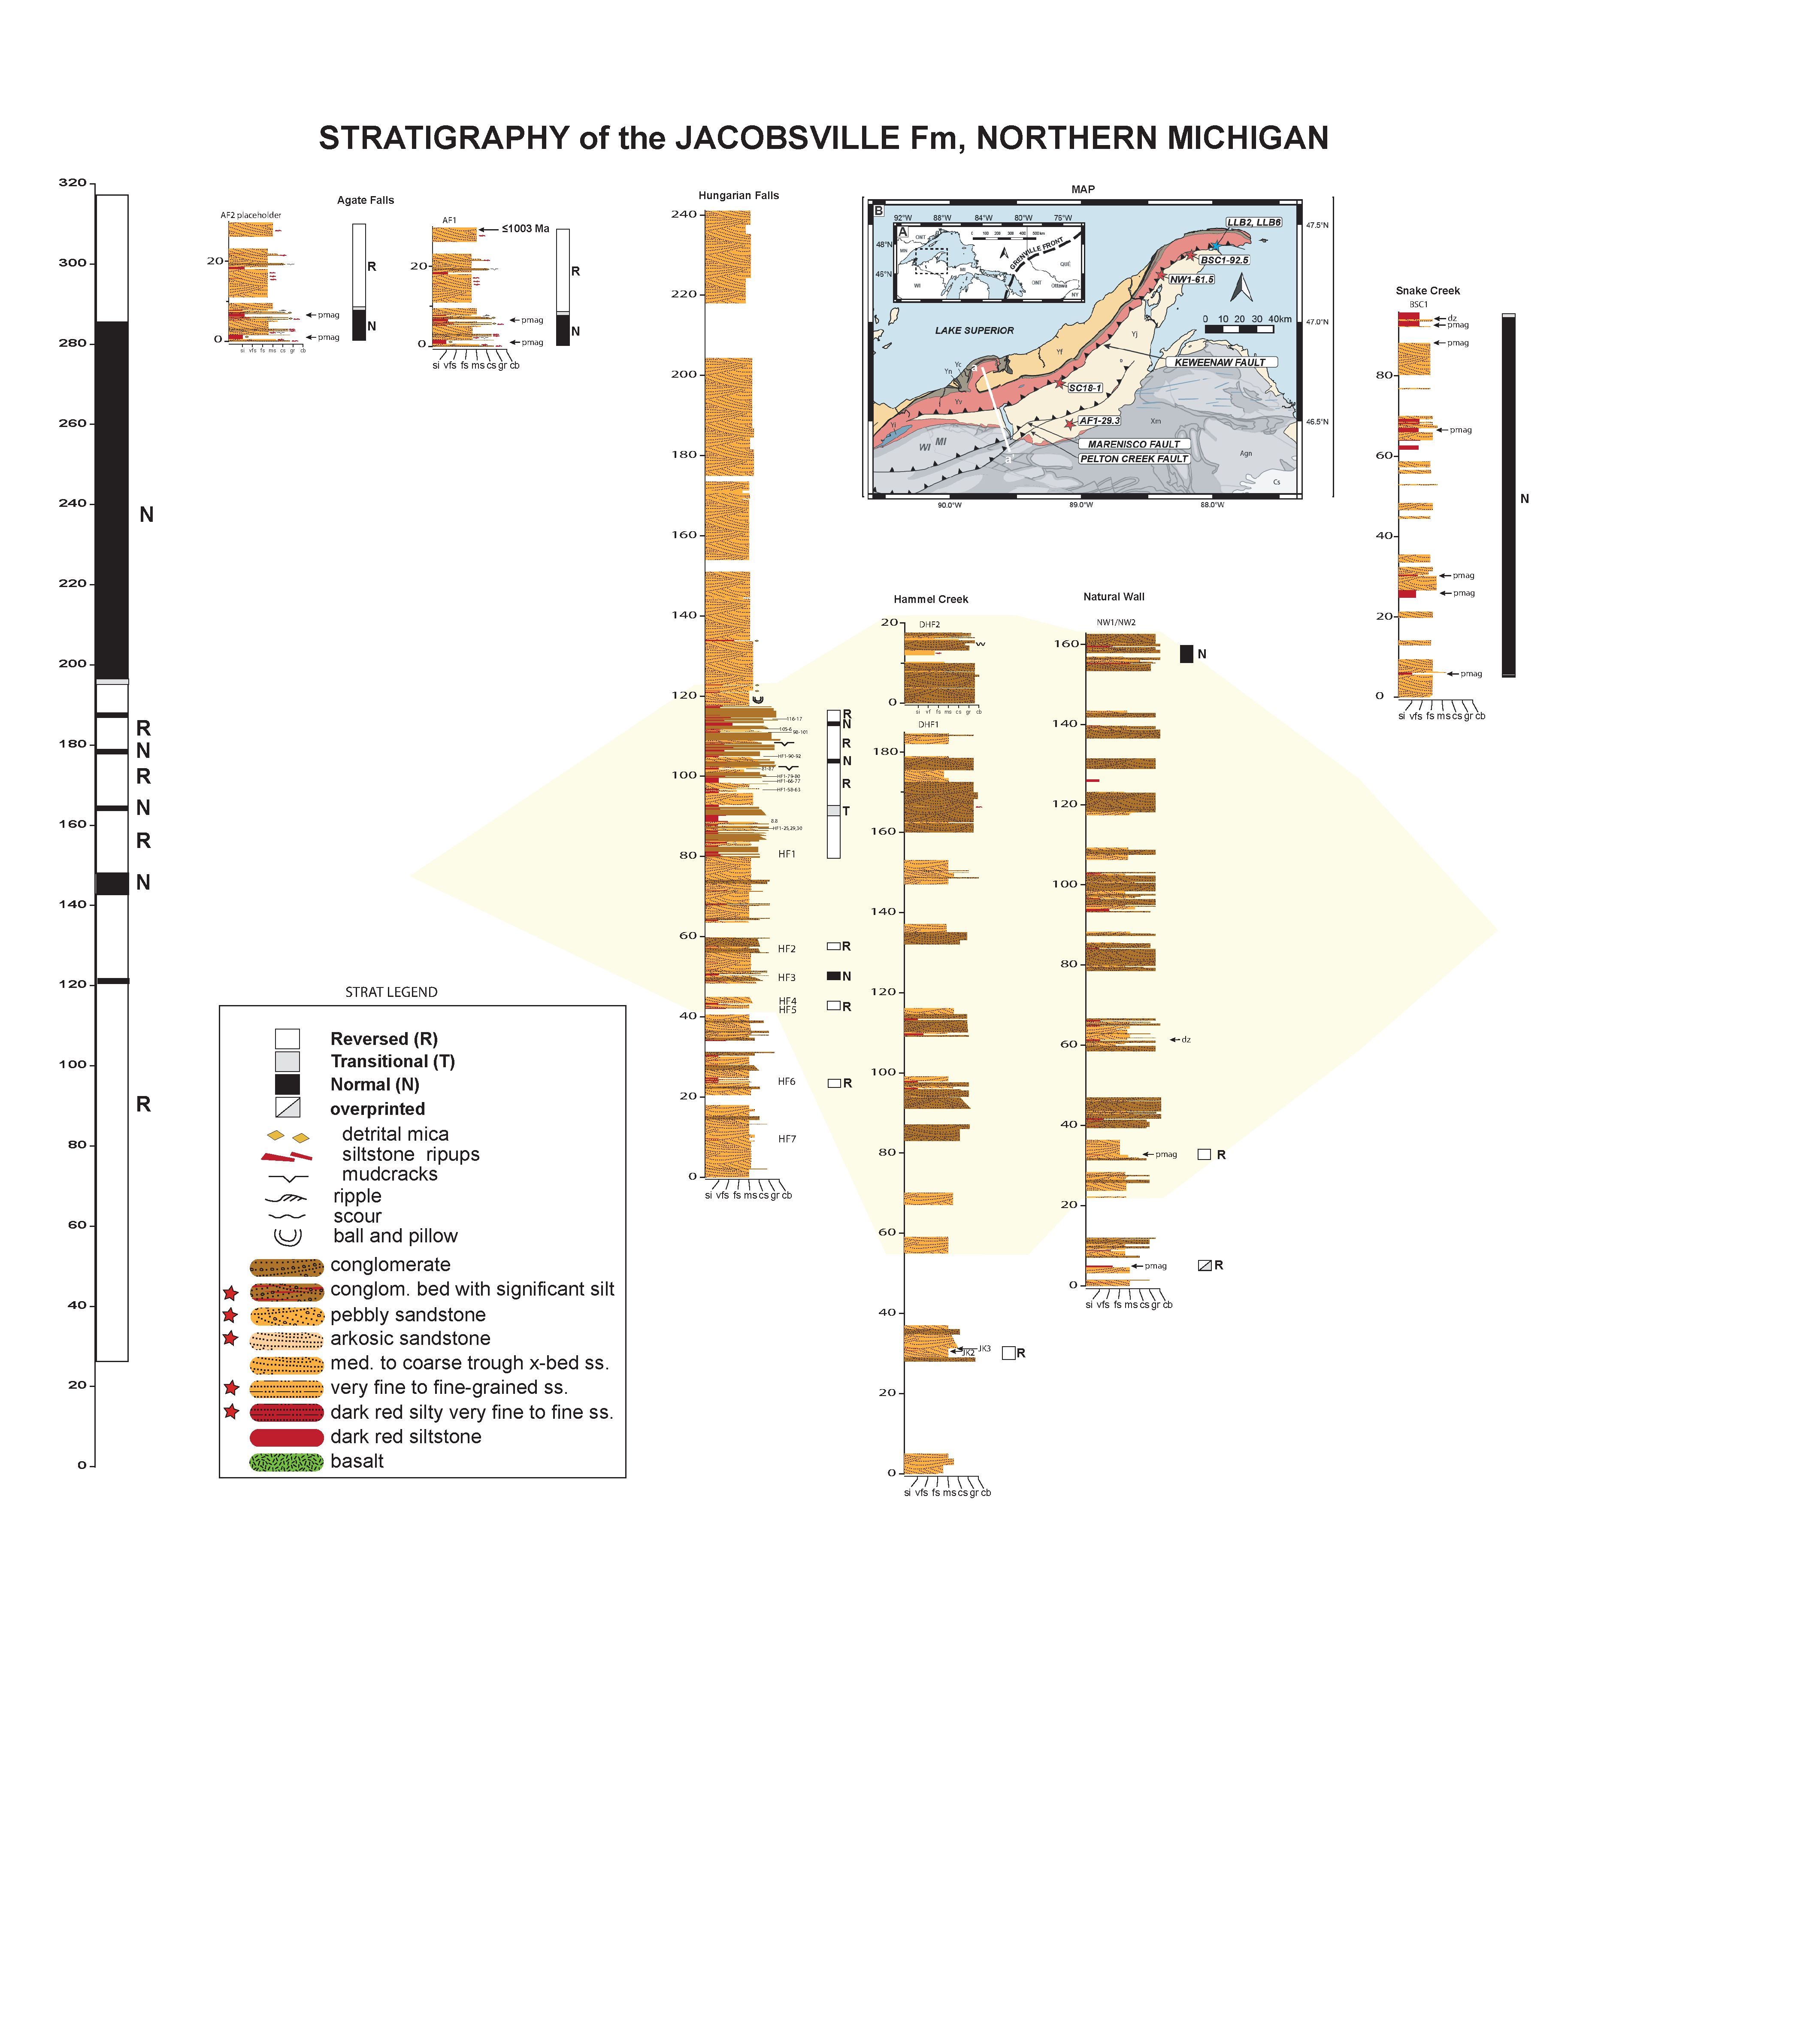
\includegraphics[width=0.9\textwidth]{Jacobsville_Sections_v3.pdf}
\caption{Tentative sedimentary stratigraphy and magnetostratigraphy for the Jacobsville Formation in northern Michigan, USA. Stratigraphic locations of paleomagnetic samples are shown in context of Jacobsville lithofacies, sedimentary structures, as well as detrital zircon maximum deposition ages developed by \citeA{Hodgin2022a}. }
\label{fig:strat_column}
\end{figure*}

% Keweenaw Fault motion post dating Jacobsville in the footwall
% Youngest DZ from jacobsvill eis about 993 Ma (sandstone creek, about a few hundred meters from the fault). 
% directly above pmag sampling at Agate falls grain B geochron date is (z2, s226, about 1000 Ma grain)

% jacobsville (985.5 from calcite in the fault and <993 from zircons) 

% Blake's current tectonic model: after MCR volcanics ca. 1084 Ma emplacement follows the deposition of the sediments (Oronto Group) copper harbor conglomerate, Nonesuch formation and the Freda formation. Then the Grenville orogenesis took off with the Ottawan phase from 1020 Ma - 10?? Ma and the Rigolet phase from 995-980 Ma. Paleosol development and the unconformity between the Jacobsville and the volcanics indicate a prolonged period of gap during which the Oronto Group in the backbulge basin where they were deposited were lost, resulting in younger Jacobsville deposition directly on top of the volcanics. The fact that in the Jacobsville has conglomerate and sandstone and siltstone facies in them supports sediment input from the eroded Oronto Group. This indicate the older boundary of the Jacobsville deposition might be closer to the Rigolet Phase than the Ottawan phase. The younger age boundary of the Jacobsville is well defined - given that the maximum deposition age from the zircons of the Jacobsville is 993 Ma and the calcite on the Keweenaw Fault is 985.5 Ma, the deposition of at least the upper portion of the Jacobsville is well constrained to be between 993 and 985 Ma. The deposition of Jacobsville in the back bulge in Laurentia interior is related to the far-field compression caused by the Grenville Orogeny. 

% This makes the Jacobsville sandstone one unique opportunity to acquire a paleomagnetic pole position within the gap between the 



\section*{Paleomagnetic methods and results}

Oriented paleomagnetic samples were collected with a portable electric drill along five stratigraphic sections of the Jacobsville Formation in norther Michigan (Fig. \ref{fig:Geologic_map}). Additional oriented cores and block samples of siltstone rip-up clasts within conglomerate lithofacies were sampled at Hungarian Falls and at Agate Falls (Fig. \ref{fig:Geologic_map}, \ref{fig:strat_column}). In order to maximize sampling of distinct time snapshots of the geomagnetic field at the time of Jacobsville deposition such that paleosecular variation can be sufficiently averaged out, we optimized for vertical stratigraphic coverage such that each sample constitutes a paleomagnetic site considering that a paleomagnetic site (which ideally captures a single snapshot of the local geomagnetic field) is a particular bed in a sedimentary sequence. Red fine-grained sandstone to shaly siltstone layers were preferentially sampled as they tend to have lower permeability and are less susceptible to diagenetic alteration through fluid flow than coarser grained sandstone. Care was taken to avoid samples containing reduction spots. Paleomagnetic cores and blocks were oriented using a magnetic compass and a sun compass whenever possible. Sun compass data were preferentially used when available. A total of 379 specimens including 30 intraclasts where collected for paleomagnetic study. The specimens underwent stepwise thermal demagnetization at the UC Berkeley Paleomagnetism Lab using an ASC demagnetizer (residual fields $<$10 nT) with measurements made on a 2G DC-SQUID magnetometer. The demagnetization protocol had high-resolution approaching the Ne\'el temperature of hematite (5 \textdegree C to 2 \textdegree C) (Fig. \ref{fig:Intraclast_pmag}). Demagnetization results are plotted in Figure \ref{fig:in_situ_pmag}A by locality. All paleomagnetic data are available to the measurement level in the MagIC database (https://earthref.org/ MagIC/; THIS LINK IS AVAILABLE TO REVIEWERS AND WILL BE UPDATED WHEN A DOI IS AVAILABLE).

\begin{figure*}[h!]
\centering
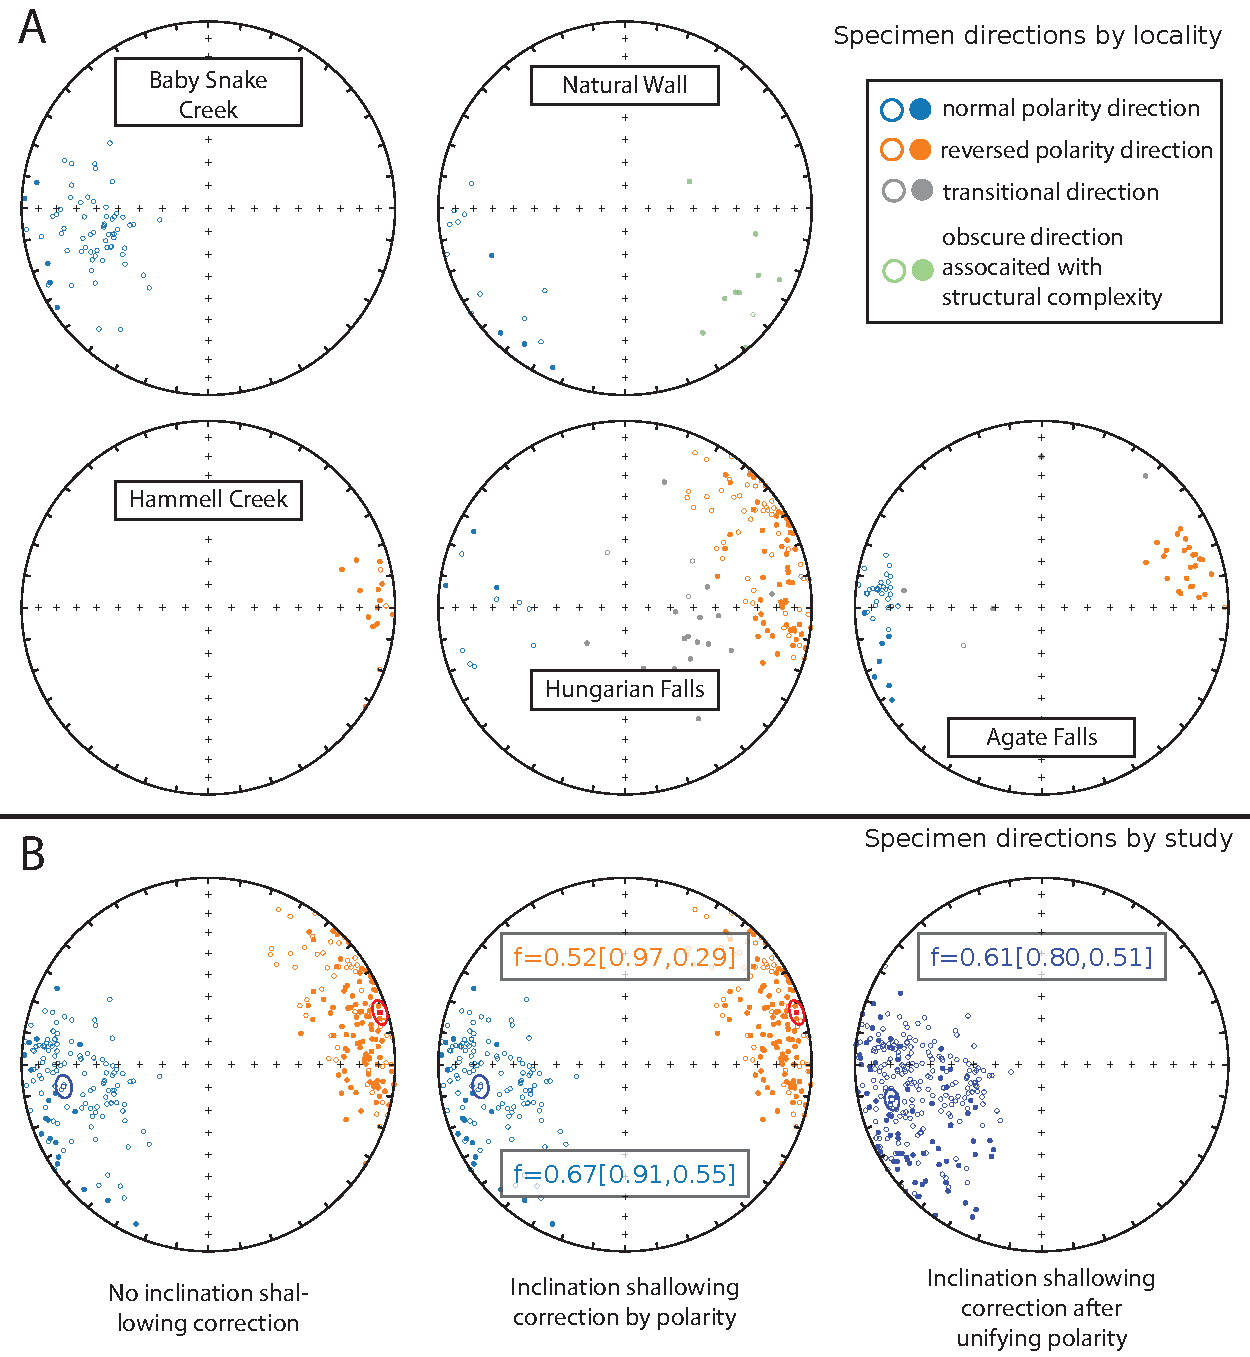
\includegraphics[width=\textwidth]{in_situ_pmag.pdf}
\caption{}
\label{fig:in_situ_pmag}
\end{figure*}


\subsection*{Paleomagnetic field test}

\subsubsection*{Fluvial intraclast conglomerate test}

Similar to the thermal demagnetization result of the hematite-bearing fluvial intraclasts of the Freda Formation \cite{Swanson-Hysell2019b}, the siltstone rip-up clasts of the Jacobsville Formation typically reveal two distinct magnetization components (Fig. \ref{fig:Intraclast_pmag}). One component show similar vector orientations amongst intraclasts and was typically removed up to 640-655 \textdegree C (Fig. \ref{fig:Intraclast_pmag}). This indicates that it is likely a chemical remanent magnetization acquired through growth of secondary hematite in pore spaces following redeposition of the clasts. After removal of this component, further thermal demagnetization with small step increments at higher temperatures up to $\sim$689 \textdegree C often reveal an origin-trending component (Fig. \ref{fig:Intraclast_pmag}). In the data from the clasts, there is typically a significant directional change in specimen magnetization between the mid-temperature component and the high-temperature component and as a result, 28 out of 30 intraclast specimens could be fit with distinct mid-temperature and high-temperature least squares lines \cite{Kirschvink1980a}. Distinct from the well-grouped mid-temperature component directions, the high-temperature directions of the intraclasts are dispersed and the null hypothesis of randomness cannot be rejected at the 95\% confidence level (n=6 for intraclasts at Agate Falls and n=22 for intraclasts at Hungarian Falls; Fig. \ref{fig:Intraclast_pmag}; \citeA{Watson1956a}). This indicates that the component is held by detrital hematite grains during initial formation of the clasts prior to erosion and redeposition. 


\begin{figure*}[h!]
\centering
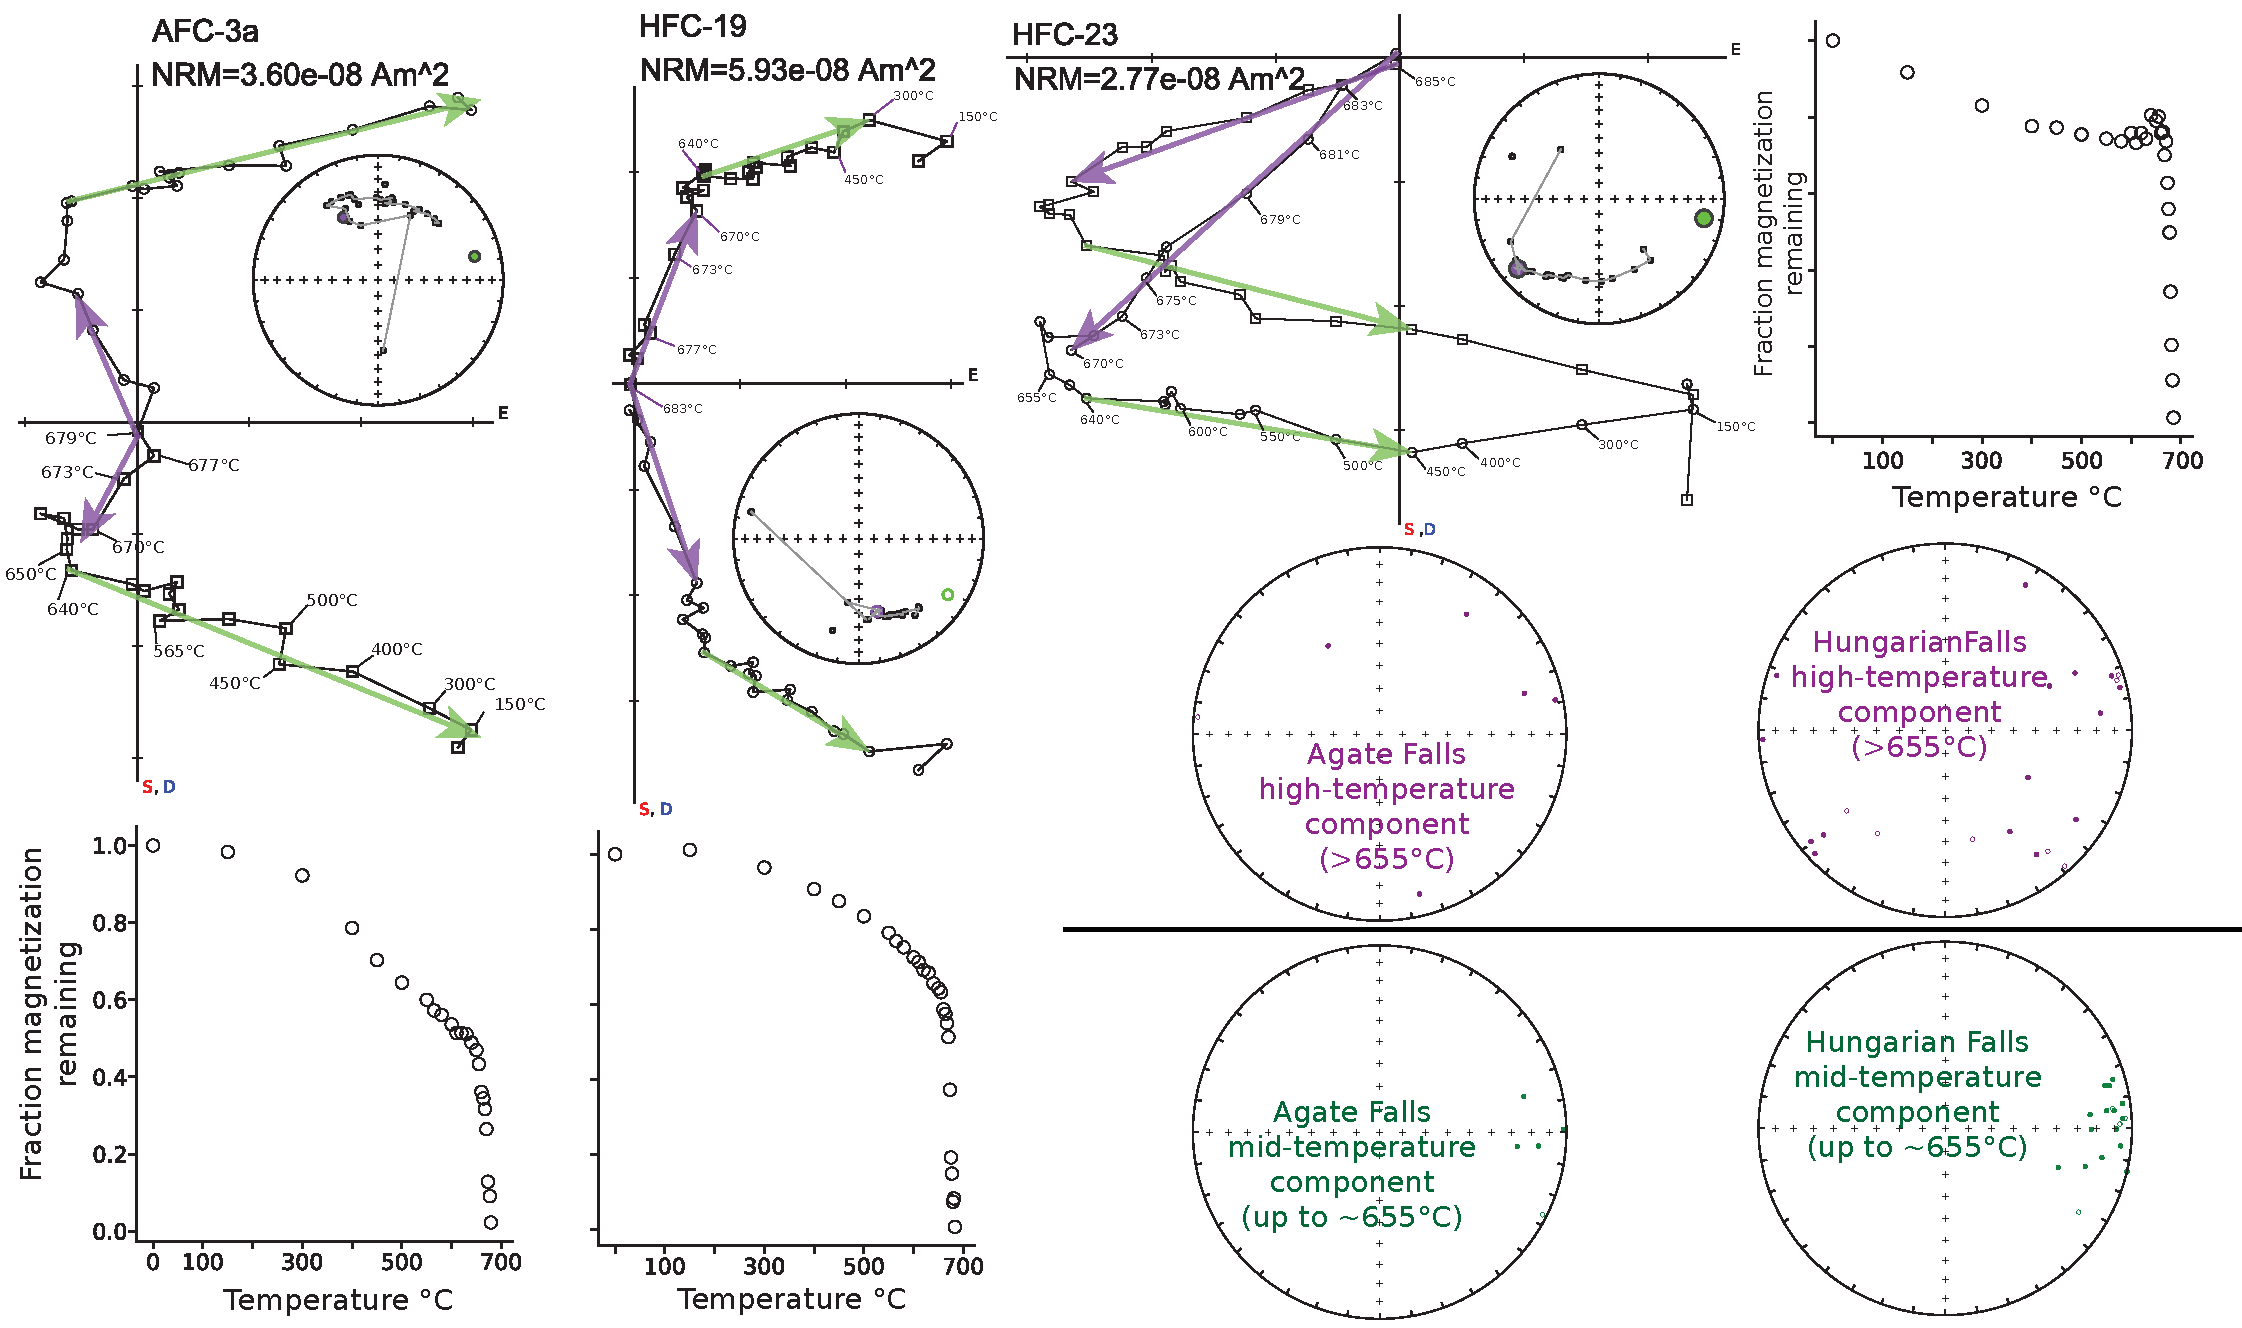
\includegraphics[width=\textwidth]{Intraclast_pmag.pdf}
\caption{Paleomagnetic data from fluvial rip-up clasts of the Jacobsville Formation reveal a mid-temperature component that typically unblocks prior to 655 \textdegree C and a high-temperature component that typically unblocks up to 689 \textdegree C. The components are present as varying fractions of the overall remanence as seen in the three individual clasts shown on vector orthogonal plots and measurement-level equal area plots in tilt-corrected coordinates (developed using PmagPy; \citeA{Tauxe2016a}). The direction of the mid-temperature component is shown as green arrows on the vector component plots and green circles on the equal area plots, while the high-temperature component is shown with purple symbols. The mid-temperature component has a similar direction among the clasts as can be seen on the summary equal area plots. In contrast, the high-temperature component directions (purple) are dispersed and pass a randomness test of \citeA{Watson1956a}. NRM = natural remanent magnetization; AFC = Agate Falls clasts; HFC = Hungarian Falls clasts.}
\label{fig:Intraclast_pmag}
\end{figure*}

\subsubsection*{Fold test}

A total of 70 specimens yielded interpretable high-temperature paleomagnetic remanence component throughout the stratigraphic section at Baby Snake Creek (Fig. \ref{fig:Geologic_map}, \ref{fig:in_situ_pmag}). The tilt-corrected remanence directions are all of normal polarity and show a dominantly southwest declination and upward-pointing inclination (Fig. \ref{fig:in_situ_pmag}). The directions in geographic coordinates yield a bootstrap fold test \cite{Tauxe1994a} result that shows the 95\% confidence bounds for the best grouping of the directions from the two limbs of the fold is achieved between 55\% and 92\% unfolding. Although the 95\% confidence bounds exclude 100\% unfolding, that the grouping of the directions become much tighter than they were in geographic coordinates when significant unfolding is applied suggest the high-temperature component from Baby Snake Creek was likely acquired pre-folding. The non-ideal unfolding test could be a result of overlapping unblocking temperatures of detrital and pigmentary hematite in red beds of Baby Snake Creek or complex folding regime near the Keweenaw Fault or a combination of the two. 

\begin{SCfigure*}
\centering
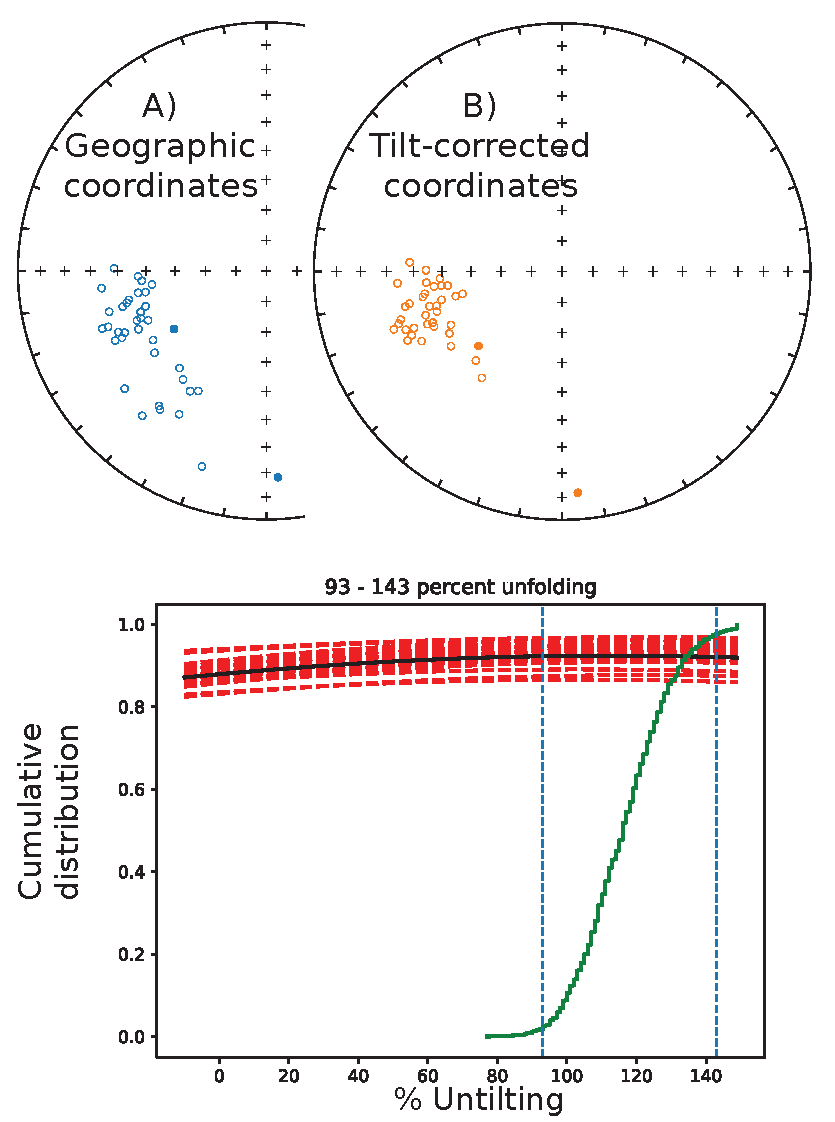
\includegraphics[width=0.5\textwidth]{SC1_fold_test.pdf}
\caption{Bootstrap paleomagnetic fold test \cite{Tauxe1994a} of the detrital remanent magnetization remanence directions recorded by specimens from Baby Snake Creek. Although the directional data set becomes more tightly grouped than in geographic coordinates when applying 55\%-92\% unfolding, both geographic and 100\% unfolded coordinate systems are excluded at the 95\% confidence level. }
\label{fig:Intraclast_pmag}
\end{SCfigure*}

\subsection*{Tentative magnetostratigraphy}
\label{magstrat}
With the insights gained from the thermal demagnetization results of the Jacobsville fluvial intraclasts, we next isolate the high-temperature magnetization component from the mid-temperature component for all in situ specimens that were collected along the five localities in northern Michigan (Fig. \ref{fig:Geologic_map}). The resultant high-temperature component directions are plotted by locality in Fig. \ref{fig:in_situ_pmag}. These results show dual polarities recorded by the Jacobsville Formation (Fig. \ref{fig:in_situ_pmag}), consistent with the observation of \citeA{Roy1978a}. Furthermore, our new data show that the Jacobsville Formation recorded more than one geomagnetic field polarity reversal and a tentative magnetostratigraphy may be constructed (Fig. \ref{fig:in_situ_pmag}). 

At Agate Falls (Fig. \ref{fig:Geologic_map}), multiple hematite-rich, detrital mica-bearing siltstone layers occur through a $\sim$30-meter strata incised by the running Middle Branch Ontonagon River. 68 paleomagnetic samples were collected on both sides of the river through overlapping stratigraphic sections (Fig. \ref{fig:strat_column}). A single transition from normal to reversed polarity is observed through the sections from bottom to top with a few strata in the middle of the section capturing transitional field directions (Fig. \ref{fig:strat_column}, \ref{fig:in_situ_pmag}). 

At Hungarian Falls (Fig. \ref{fig:Geologic_map}), numerous hematite-rich siltstone to fine-grained silty sandstone layers were deposited. The siltstone and silty fine-grained sandstone layers can capture a relatively rich set of information from the paleomagnetic field variations compared to coarser-grained lithologies at other localities (Fig. \ref{fig:strat_column}). Throughout $\sim$240 meters of stratigraphy, a total of 158 samples were collected for paleomagnetic study. At stratigraphic height of $\sim$24 meters (Fig. \ref{fig:strat_column}), 8 samples from a $\sim$0.5-meter-thick siltstone layer record a reversed polarity (easterly declination and shallow inclination; horizon HF6). At stratigraphic level $\sim$42 meters (HF5; Fig. \ref{fig:strat_column}), 4 samples were collected through a $\sim$0.2 m siltstone horizon including one specimen from near the base of the layer and three specimens near the top of the layer. The high-temperature remanence component from the three specimens near the top all record a reversed polarity whereas the specimen collected near the base show a westerly declination. While more samples are needed to test whether the westerly declination recorded by the single sample is a result of the geomagnetic field having completely flipped polarity from that recorded by horizon HF6 or a result of transient unstable field, this anomalous direction indicates that the geomagnetic field did not stay consistent throughout the time of deposition of this horizon. As a result, we tentatively mark a period of transitional field near the base of horizon HF5 in Fig. \ref{fig:strat_column}. A reversed polarity field seems to have been maintained as 5 samples from horizon HF4 consistently record easterly directions similar to those recorded by samples near the top of HF5 (Fig. \ref{fig:strat_column}). However, a geomagnetic field polarity reversal happened between the deposition of siltstone layers of HF4 and HF3, as 7 samples from HF3 all record normal-polarity directions, antipodal to those of samples of HF4. Subsequently, the field appears to flip again back to reversed polarity, as is shown by 7 samples from HF2 higher above the section (Fig. \ref{fig:strat_column}). Through the $\sim$35-meter-thick horizon of HF1 characterized by numerous siltstone to fine-grained sandstone layers interbedded with coarser-grained sandstone and conglomerate, magnetic polarity reversals of R-N-R-N-R were recorded (Fig. \ref{fig:strat_column}). 

The Natural Wall ravine and Hammell Creek are in close proximity toHungarian Falls (Fig. \ref{fig:Geologic_map}) and the sedimentary facies characterized by trough cross-bedded sandstone and conglomerates are similar to the basal $\sim$120 meters of the section at Hungarian Falls (Fig. \ref{fig:strat_column}). Since only a couple of siltstone to fine-grained sandstone horizons were sampled at these two localities, we tentatively correlate the stratigraphic sections at these three localities based on their sedimentary facies and magnetic polarities (Fig. \ref{fig:strat_column}). At Hammell Creek, 14 samples from two siltstone layers near the base of the section are of reversed polarities, consistent with the reversed-polarity layers near the base of Hungarian Falls. Near the top of the Natural Wall section, consistent normal-polarity directions are recorded by 15 samples. This normal polarity could be coeval with one of the normal-polarity periods recorded at Hungarian Falls, or it could indicate an additional polarity reversal from reversed to normal polarity that happened after the deposition of the youngest reversed strata at Hungarian Falls (Fig. \ref{fig:strat_column}). Near the base of the stratigraphic section at Natural Wall (Fig. \ref{fig:strat_column}), the strata are steeply tilted or overturned (Fig. \ref{fig:Field_photo}). Tilt-corrected paleomagnetic directions from samples collected from these strata show dominantly southeasterly declinations that are distinct from either normal- or reversed-polarity directions higher along the strata or at Hungarian Falls. Possible causes of such distinct directions could be related to transitional fields associated with geomagnetic field polarity reversals or complications in the tilt correction such as noncylindrical folding or multiple tilting episodes. 

A total of 70 specimens yielded interpretable high-temperature paleomagnetic remanence component throughout the stratigraphic section at Baby Snake Creek (Fig. \ref{fig:Geologic_map}, \ref{fig:in_situ_pmag}). The remanence directions recorded by red beds within the steeply folded basal section and within the flat-lying top portion of the section pass a bootstrap fold test (Supporting Information; \citeA{Tauxe1994a}). The remanence directions are all of normal polarity and show a dominantly southwest declination and upward-pointing inclination (Fig. \ref{fig:in_situ_pmag}). 

Given that multiple geomagnetic field reversals occurred during the deposition of the Jacobsville Formation, the development of amagnetostratigraphy should be possible and could be useful for future regional and global studies. However, challenges exist in correlating the stratigraphic sections measured at the five localities in this study due to the lateral variability of the paleodepositional environment associated with the variable paleotopographic relief of the Precambrian surface upon which the Jacobsville Formation was deposited \cite{Hamblin1958a, Kalliokoski1982a}. In particular, there may not be a unique solution in reconstructing the relative stratigraphic positions of the strata at Baby Snake Creek and Agate Falls with respect to the other three sections in central Keweenaw Peninsula due to geographical separation (Fig. \ref{fig:Geologic_map}, \ref{fig:strat_column}). However, at both Baby Snake Creek and Agate Falls, the sedimentary strata are dominated by siltstone to cross-bedded sandstone and are lacking significant amount of conglomerate facies as seen near Hungarian Falls. This could be consistent with the interpretation that these strata were deposited as the Jacobsville basin of the Grenvillian foreland system resulted from lithospheric flexure induced by orogenic loading has been partially filled. Recent geologic mapping efforts near Baby Snake Creek have found evidence for the Jacobsville Formation onlapping the Midcontinent Rift volcanics that were previously faulted via en echelon segments\cite{Tyrrell2019a, Mueller2021a}. The unconformable contact between the sediments and the volcanics, instead of faulted contact typically observed near Hungarian Falls where the basal Jacobsville Formation is folded and faulted against the volcanics, indicate that the deposition of the Jacobsville Formation near the northern end of Keweenaw Peninsula likely post-date some episodes of motion along the Keweenaw Fault. Therefore, we interpret that the normal-polarity strata at Baby Snake Creek could be stratigraphically the youngest amongst the five localities, although a possibility that they instead are near the bottom of the stratigraphy and record the normal Keweenawan Superchron cannot be ruled out \cite{Driscoll2016b}. 

Overall, the multiple geomagnetic field polarity reversals recorded by the Jacobsville Formation constrain the maximum range of the Keweenawan normal superchron \cite{Driscoll2016b} to be between ca. 1100 (Mamainse Point Volcanics; \cite{Swanson-Hysell2019a}) to ca. 992 Ma (maximum deposition age of Jacobsville Formation; \cite{Hodgin2022a}). 



\begin{figure*}[h!]
\centering
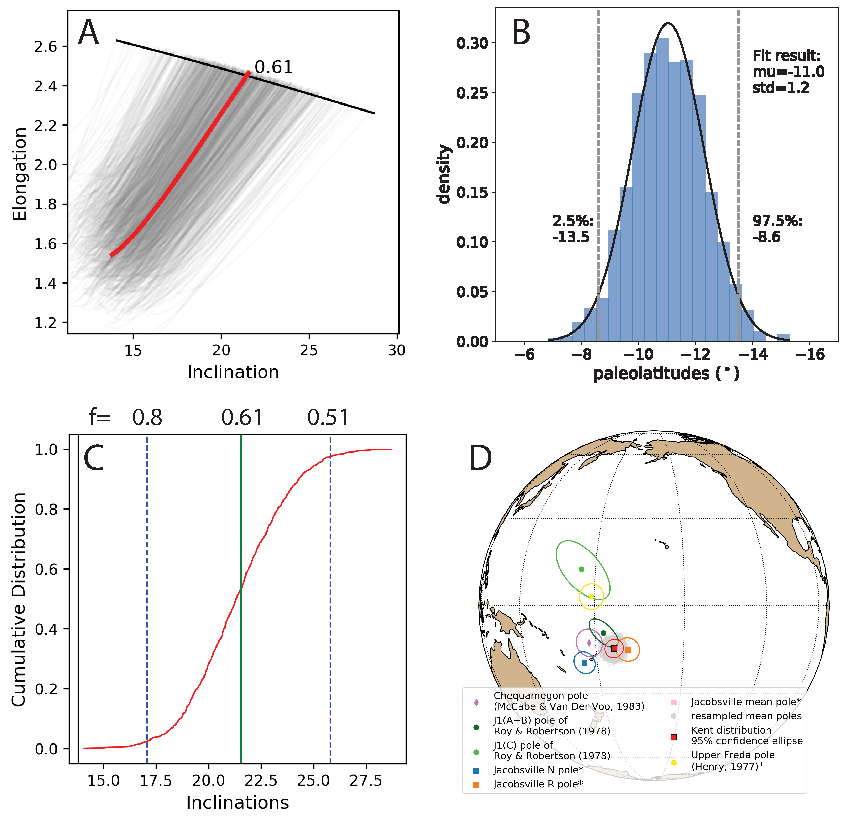
\includegraphics[width=\textwidth]{EI_results.pdf}
\caption{}
\label{fig:EI_results}
\end{figure*}

\begin{figure*}[h!]
\centering
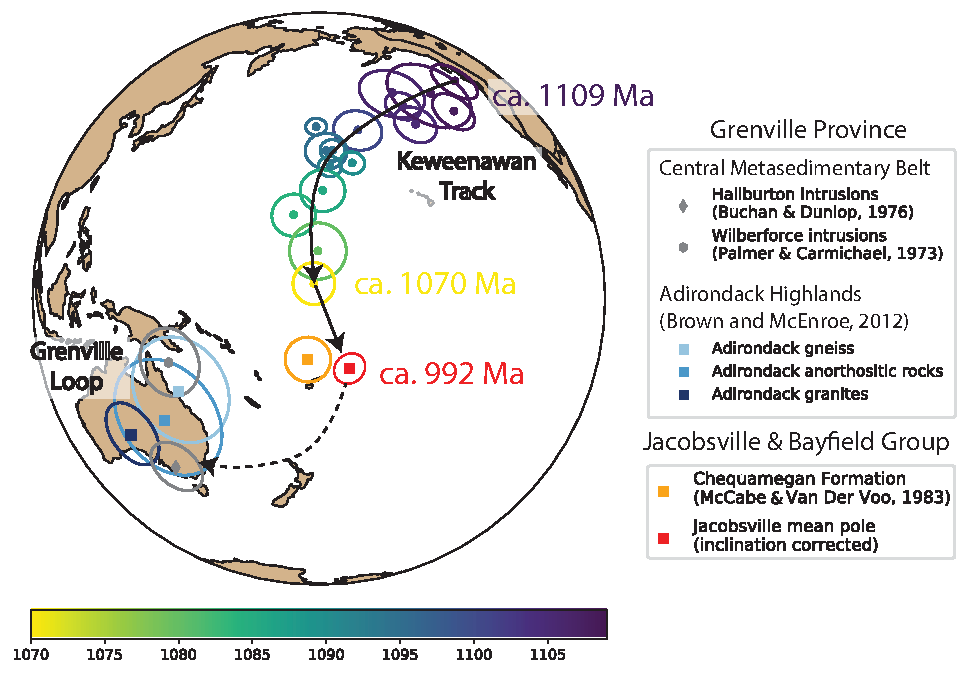
\includegraphics[width=\textwidth]{Jacobsville_pole_plot.pdf}
\caption{}
\label{fig:pole_plot}
\end{figure*}



\section*{Discussion}

\subsection*{Inclination shallowing correction}

Although igneous and sedimentary rocks associated with the North American Midcontinent Rift provided high-resolution record of the ca. 1110 to 1070 Ma Keweenawan Track which is the apparent polar wander path (APWP) for Laurentia in the late Mesoproterozoic, high-quality paleogeographic constraints is lacking thereafter since magmatism in the interior of Laurentia entered a protracted quiescence period until the emplacement of the ca. 780 Ma Gunbarrel large igneous province \cite{Harlan2003a}. The new paleomagnetic data developed from the Jacobsville Formation presents an opportunity to extend the Keweenawan Track toward the early Neoproterozoic as its maximum deposition age has been tightly constrained to be ca. 992 Ma through high-precision U-Pb detrital zircon geochronology \cite{Hodgin2022a}. 

However, inclination bias associated with sedimentary paleomagnetic directions need to be corrected when synthesizing poles. Rotation of grains during sediment deposition and compaction during early diagenesis can result in the acquisition of a detrital remanent magnetization that is more shallowly inclined relative to the local geomagnetic field in which it was acquired \cite{King1955a, Tauxe2005a, Kodama2012a}. This effect can be summarized as: 
\begin{equation*}
\textup{tan}(I_o) = f\textup{tan}(I_f)
\end{equation*}
where $f$ represents the amount of inclination shallowing, $I_o$ represents the observed inclination, and $I_f$ represents the inclination of the field in which the magnetization was acquired. If uncorrected, shallower inclinations obtained from sedimentary rocks can result in erroneously low estimates of paleolatitudes, biasing paleogeographic reconstructions \cite{Domeier2012a}. Methods for correcting sedimentary inclination bias include laboratory-based measurements of magnetic mineral fabrics \cite<e.g.>{Kodama1992a, Bilardello2015a}, as well as statistical methods based on the evaluation of the deviation of observed virtual geomagnetic pole (VGP) distribution patterns from an assumed paleosecular variation model (the ``elongation/inclination" [E/I] method of \citeA{Tauxe2004b}). When a large number of sedimentary paleomagnetic samples (typically n$>$100) capture an extensive period of time such that the paleosecular variation is sufficiently averaged, the E/I method can give accurate estimates and is less labor-intensive than methods based on mineral fabric measurements. In the ca. 1.1 Ga Midcontinent Rift, \citeA{Pierce2022a} showed that the E/I method is effective in correcting the inclination bias recorded by a package of lava flow-bracketed fluvial red bed sediments---the Cut Face Creek Sandstone.

Inclination shallowing is also present in the fluvial red beds of the Jacobsville Formation. Scatter of the specimen detrital remanence directions in geographic coordinates show dispersion of remanence vectors parallel to the bedding plane, indicating the directions are likely shallowed along the bedding-perpendicular plane (Fig. \ref{fig:in_situ_pmag}; \citeA{Tauxe2004b}). Since the deposition of the Jacobsville Formation span over geomagnetic field reversals, it is of interest to investigate the amount of inclination shallowing associated with the normal (n=130) and the reversed (n=148) polarity respectively. Applying the E/I method on the normal polarity directions yields an estimated $f$ value of 0.67 with 95\% bootstrap uncertainty bounds from 0.91 to 0.55 (Fig. \ref{fig:in_situ_pmag}B). On the other hand, directions of reversed polarity yields an estimated $f$ factor of 0.52 with more uncertainties ranging from 0.97 to 0.29 (Fig. \ref{fig:in_situ_pmag}B). Although the estimated $f$ value for the reversed-polarity directions has large statistical uncertainty bounds, the uncertainties are likely associated with the overall shallow inclinations and distributions of directions in both upper and lower hemispheres (Fig. \ref{fig:in_situ_pmag}B). Therefore, inclination corrections do not result in significant changes in the mean reversed direction. In addition, directions of the two polarities do not pass a reversal test \cite{McFadden1990a, Tauxe2010a}, regardless of whether inclination correction is applied. 

One interpretation of the polarity discrepancy could be that the deposition of the Jacobsville Formation was protracted such that the sediments at Hungarian Falls whose detrital remanence dominate reversed polarity records was deposited prior to those at Baby Snake Creek which dominate the normal polarity records (Fig. \ref{fig:in_situ_pmag}). This is consistent with the magnetostratigraphic interpretation that Baby Snake Creek section is younger than the Hungarian Falls section (Fig. \ref{fig:strat_column}). Field observations of \citeA{Tyrrell2019a} and \citeA{Mueller2021a} near Bete Grise Bay, which is only $\sim$10 km east to Baby Snake Creek (Fig. \ref{fig:Geologic_map}), show unconformable onlap of the Jacobsville Formation on top of Midcontinent Rift volcanics that have experienced significant thrusting, deformation. At some locations, paleosol development has been found on top of the Midcontinent Rift basalt along the segmented Keweenaw Fault branches prior to the deposition of the Jacobsville sediments. This is in contrast with the faulted contact between the Jacobsville Formation and the volcanics to the south where the Jacobsville Formation is often folded against the volcanics (Fig. \ref{fig:Geologic_map}). U-Pb calcite geochronology and thermometry confirm that the final $\sim$2 km vertical displacement along the Keweenaw Fault occurred during the ca. 980 Ma Rigolet phase of the Grenvillian Orogeny whereas the majority of the fault motion likely occurred during the ca. 1050 Ma Ottawan phase \cite{Hodgin2022a}. We interpret that it is most likely that deposition of the Jacobsville Formation initiated close to the Rigolet phase of the Grenvillian Orogeny with progressive sediment transportation to the northwest as the Grenville back-bulge basin propagated toward the interior of Laurentia \cite{Hodgin2022a}. As a result, we hypothesize that the sediments at Baby Snake Creek likely records a slightly younger pole position with a more southerly paleolatitude than those near Hungarian Falls, indicating Laurentia's plate motion toward the south (Fig. \ref{fig:EI_results}). However, we cannot rule out an alternative interpretation that the sediments at Baby Snake Creek are coeval or older than some of the sediments to the south, as the basal Jacobsville Formation at Baby Snake Creek is folded against the Midcontinent Rift volcanics. Further field mapping and geochronological constraints are needed to test this hypothesis. 

% An alternative interpretation to the polarity discrepancy could be that there are insufficient samples such that either or both polarities are not average for secular variation. 
Overall, both inclination-corrected polarities recorded by the Jacobsville Formation show mean pole positions in the southern hemisphere with respect to today's continental configuration (normal polarity longitude=175.1\textdegree E, latitude=19.1\textdegree S, A95=3.8\textdegree; reversed polarity longitude=191.1\textdegree E, latitude=14.5\textdegree S, A95=3.9\textdegree; both are corrected for inclination shallowing; Fig. \ref{fig:EI_results}). The two pole positions are distinct from the youngest poles developed from rocks of the Midcontinent Rift (Fig. \ref{fig:EI_results}). Despite that the Jacobsville sedimentation span over geomagnetic field reversals, the large arc distance between either polarity of the Jacobsville Formation and the pole of the ca. 1070 Ma upper Freda Formation is consistent with the interpretation that the onset of deposition of the Jacobsville Formation at the five studied localities post-date the youngest member of the Oronto Group sediments by tens of millions of years. 

\subsection*{The Jacobsville paleomagnetic pole}
To succinctly summarize a paleomagnetic pole for the ca. 992 Ma Jacobsville Formation, we combine the directions of both polarities and reassess the amount of inclination shallowing of the combined directional dataset (Fig. \ref{fig:in_situ_pmag}). The resultant estimate for the $f$ value is 0.61 with a bootstrap 95\% uncertainty range for the $f$ value between 0.80 to 0.51, which overlaps with the uncertainty ranges of directions associated with either polarity (Fig. \ref{fig:in_situ_pmag}). The $f$ value of 0.61 is strikingly close to the value of 0.59 which is a calculated mean value of a compilation of inclination shallowing factor for hematite-bearing rocks derived by \cite{Bilardello2010b}. The Fisher mean paleomagnetic pole associated with the combined directions is shown in Fig. \ref{fig:EI_results} (pole longitude= 186.3\textdegree E, pole latitude= 14.3\textdegree S, A95= 2.5\textdegree). 

\citeA{Pierce2022a} discussed that as inclination shallowing processes usually do not bias the recorded declination, it would typically result in asymmetric uncertainties in the recorded paleomagnetic pole position with more uncertainties in paleolatitues than paleolongitudes. The asymmetric uncertainties in the mean pole position thus violate the assumption of the Fisher distribution \cite{Fisher1953a} where uncertainties are circularly distributed about a mean vector. Instead, the spherical asymmetric bivariate Kent distribution \cite{Kent1982a} is more appropriate for incorporating uncertainties associated with inclination shallowing in reported sedimentary paleomagnetic poles. We follow the approach of \citeA{Pierce2022a} who extended the E/I method of \citeA{Tauxe2004b}. First we take all estimated $f$ values from the bootstrap results of the E/I algorithm and apply each value to correct all Jacobsville detrital remanence directions (with the reversed directions flipped to antipodes). Then we calculate the Fisher statistics for each of the inclination-corrected mean pole. Finally, we perform a Monte Carlo approach to generate 100 resamples of each Fisher mean pole. As a result, the distribution of the resampled mean pole positions have an elongated distribution which represents more uncertainty associated with paleolatitudes of Laurentia than paleolongitudes (Fig. \ref{fig:EI_results}). The distribution of paleolatitudes of the resampled mean poles can be well-approximated by a normal distribution (Fig. \ref{fig:EI_results}). We use the Kent distribution to parameterize the 95\% confidence ellipse of the distribution of the resampled mean poles (mean longitude=186.4\textdegree E, mean latitude=14.2\textdegree S, major axis longitude=262.5, major axis latitude=43.5, major axis magnitude=3.3\textdegree, minor axis longitude=110.0, minor axis latitude=43.0, minor axis magnitude=3.0\textdegree; Fig. \ref{fig:EI_results}). As is shown in Fig. \ref{fig:EI_results}, although the Kent uncertainty ellipse has significant overlap with the circular uncertainty range calculated by the Fisher statistics due to the overall low paleolatitude of the Jacobsville basin, the Kent ellipse informs more uncertainty along the great circle path between the mean pole position and the locality of the basin as it incorporates the uncertainties in the amount of inclination shallowing within the sediments. 

\citeA{Roy1978a} isolated the detrital magnetization component via alternating-field, thermal, and chemical ``cleaning" demagnetization on a suite of Jacobsville red beds near Keweenaw Peninsula (their area A), the town of Marquette (area B), and Sault Ste Marie (area C). Although least-squares principal component analyses was not a routine approach in fitting paleomagnetic directions at the time, that study had success in removing the present day local field overprint and was able to resolve a magnetic polarity transition at one locality. The mean paleomagnetic pole position calculated from the interpreted primary magnetic remanence from rocks of the Keweenaw Peninsula and Marquette (J1 A+B pole; pole longitude=183\textdegree E, pole latitude=9\textdegree S, dp=3\textdegree, dm=6\textdegree; no inclination correction; Fig. \ref{fig:EI_results}; \citeA{Roy1978a}) is in the southern hemisphere and the uncertainty ellipse overlaps with that of the mean pole from this study (Fig. \ref{fig:EI_results}. However, their mean pole developed from red beds near Sault Ste Marie is in the northern hemisphere with a latitude of 12\textdegree N (Fig. \ref{fig:EI_results}). Despite the large uncertainty ellipse associated with this mean pole position, it is distinct from the mean pole position from Jacobsville rocks of the Keweenaw Peninsula and Marquette. Instead, it overlaps with the mean pole position of the ca. 1070 Ma Upper Freda Formation (Fig. \ref{fig:EI_results}; \citeA{Henry1977a}). We hypothesize that the red beds collected by \citeA{Roy1978a} in Sault Ste Marie area are likely Freda-equivalent sediments, instead of being a part of the Jacobsville Formation. 

Deposition of the Bayfield Group sediments west to the Keweenaw Peninsula has been hypothesized to be coeval with the Jacobsville Formation but chronological constraints have been lacking. Our new paleomagnetic data from the Jacobsville Formation reaffirms that the pole positions of the the Chequamegon Sandstone of the Bayfield Group and the Jacobsville Formation are close albeit distinct (Fig. \ref{fig:EI_results}). Given that the paleomagnetic pole from the Chequamegon Sandstone of the Bayfield Group (pole longitude=177.7\textdegree E, pole latitude=12.3\textdegree S, A95=4.6\textdegree; \citeA{McCabe1983a}) was calculated without applying inclination correction, the two formations could have even closer a temporal association than the current paleomagnetic pole configuration appears (Fig. \ref{fig:EI_results}). In addition, the fact that only reversed polarity directions were recovered from the Chequamegon Sandstone could indicate that deposition of the sandstone collected by \citeA{McCabe1983a} could be coeval with one of the reversed polarity period recorded by the Jacobsville Formation (Fig. \ref{fig:strat_column}). To further test the temporal correlation between the sedimentary units, detailed paleomagnetic study and detrital zircon U-Pb geochronology data from the Chequamegon Sandstone are needed. 

\subsection*{Paleogeography of Laurentia in the late Proterozoic and the development of supercontinent Rodinia}

Laurentia's apparent polar wander is well constrained in the Mesoproterozoic by the Keweenawan Track thanks to the large number of paleomagnetic poles paired with high-precision geochronology from rocks of the ca. 1.1 Ga Midcontinent Rift \cite{Swanson-Hysell2019a}. In addition, the Midcontinent Rift have had simple a thermal history for their old ages, as rifting ceased prior to lithospheric separation, preserving rocks of the rift within the continental interior far from continental margin and subsequent orogenesis. Since the end of the Midcontinent Rift mamatism, igneous paleomagnetic records from the the interior of Laurentia is lacking, and data from rocks associated with the ca. 1080 to 980 Ma Grenville Orogeny have been used to infer for Laurentia's plate configuration in the late Mesoproterozoic to early Neoproterozoic \cite<e.g.>{Weil1998a, Halls2015b}. However, in contrast to rocks of the Midcontinent Rift which usually have straightforward paleomagnetic records \cite<e.g.>{Swanson-Hysell2019a}, rocks of the Grenville Province which experienced up to granulite facies metamorphism have much more complicated thermal histories and the timing of their magnetic remanence acquisition and alteration is more difficult to constrain. As is shown in Fig. \ref{fig:pole_plot}, paleomagnetic poles developed from rocks of the Grenvillian Orogeny plots near Australia with respect to today's continental configuration, forming arc distances ranging from $\sim$35\textdegree to more than 50\textdegree away from the pole of the ca. 1070 Ma Freda Formation \cite{Henry1977a}. Such large discrepancies between pole positions associated with uncertainties in the age of the magnetization of the Grenville rocks led to the controversial ``Grenville Problem"---did the Grenville rocks acquire magnetic remanence prior to the continental collision and thus the pole discrepancies are a result of significant crustal shortening (i.e. the ``two plate model"; \citeA<e.g.>{Irving1972a, Palmer1973a, Buchan1973a, Halls2015b}), or did they acquire remanence after the continental accretion and thus the southerly poles from the Grenville rocks represent Laurentia's continued motion through more recent times (i.e. the ``one plate model"; \citeA<e.g.>{Roy1978a, McWilliams1975a, Weil1998a})?

The two plate hypothesis is based on the interpretation that timing of magnetic remanence acquisition of the Grenville rocks was close to that of the Midcontinent Rift rocks \cite<e.g.>{Warnock2000a, Halls2015b}, but the lack of southerly paleomagnetic poles from the interior of Laurentia is interpreted to indicate that the Grenville rocks acquired remanence on allochthonous terranes before the final accretion to Laurentia craton. Thus, up to 4000 $\pm$ 1000 km of crustal shortening was invoked by \citeA{Halls2015b} to explain the large arc distance between the poles. 

Given the new constraints on the age and position of the Jacobsville pole (Fig. \ref{fig:pole_plot}), the two plate model would require that the majority of the crustal shortening happened after the Rigolet phase of the Grenville Orogeny, as the ca.992 Ma Jacobsville pole is still $\sim$45\textdegree\ arc distance ($\sim$5000 km) away from the paleomagnetic pole of the Haliburton intrusions \cite{Buchan1976a} and $\sim$38\textdegree\ ($\sim$4000 km) from the pole of the Wilberforce intrusions \cite{Palmer1973a} (Fig, \ref{fig:pole_plot}). However, geologic and geochronologic evidence from both within the Grenville Province \cite{Aleinikoff2021a} and from interior Laurentia \cite{Hodgin2022a} indicate that majority of the deformation in the Grenville Province and the propagation of its associated deformation in the Midcontinent Rift happened during the ca.1090-1020 Ma Ottawan phase orogeny, whereas smaller amount of convergence happened during the ca. 1010-980 Ma Rigolet phase. The lack of geological evidence for a striking amount of crustal shortening is supported by the slow average plate motion between the deposition of the upper Freda Formation and the deposition of the Jacobsville Formation (average $\sim$0.2\textdegree/Myr; Fig. \ref{fig:pole_plot}). Therefore, it is kinetically unlikely that the plate of Laurentia suddenly increased its motion during the waning phase of a collisional orogenesis in order to satisfy the Grenville pole positions. The plate kinetics interpretation based solely on paleomagnetic data and poorly constrained ages of magnetic remanence put forward by \citeA{Halls2015b} is implausible. Alternatively, the one plate model is much more straightforward in explaining the paleomagnetic pole positions of Grenville rocks as it interprets that the remanence was acquired during prolonged slow cooling of the orogeny that postdate the peak metamorphism. In contrast with the two plate model, the one plate model would predict that ages associated with the Grenville poles are much younger than ca. 980 Ma as the rocks slowly cooled after the peak metamorphism associated with the collisional orogenesis (Fig. \ref{fig:pole_plot}). 

Adopting the one plate model to explain Laurentia's late Proterozoic apparent polar wander path necessitates that the ages assigned to many paleomagnetic poles derived from Grenville rocks need to be adjusted toward younger. Abundant petrological and geochronological evidence show large portion of the Grenville Province experienced up to granulite facies metamorphism (e.g. $>$700\textdegree C). Such high peak metamorphism temperatures would result in unblocking of any remanence the rocks had acquired earlier and complete overprint by remanence acquired during cooling after the orogenesis. Previous paleomagnetic studies have found that Grenville rocks commonly have magnetite and hematite being the remanence carriers \cite<e.g.>{Ueno1975a, Alvarez1998a, Buchan1973a, Buchan1976a, Brown2012a}. Theoretical calculations have shown that magnetite which formed above its Curie temperature (580\textdegree C) in Grenville rocks subsequently acquired thermoviscous remanence \cite{Pullaiah1975a, Dodson1980a} during prolonged cooling of the orogen, whereas hematite which often occur as exsolved lamellae interfingering with ilmenite acquired thermochemical remanence via magnetic ordering of the hemo-ilmenite below the Neel temperature of hematite \cite{Burton1985a, Harrison2006b}. 

Due to the long time scales involves with thermoviscous and thermochemical origin of the magnetic remanence, it is not straightforward to interpret the natural blocking temperatures of Grenville rocks based on observations of unblocking temperatures in the lab where rocks are heated and cooled rapidly. As a result, extrapolating equivalent natural blocking temperatures from lab unblocking temperatures using theoretical models \cite{Pullaiah1975a, Dodson1980a} and pairing the temperatures with thermochronology data is necessary to determine age of the remanence. \citeA{Brown2012a} recognized that the hemo-ilmenite exsolution occur at relatively low temperatures during cooling of the orogen and interpreted their new paleomagnetic data from rocks of the Adirondack Mountains, US, in context of recent understanding of the hemo-ilmenite phase diagram. That study assigned an age of ca. 960 Ma to a paleomagnetic pole developed from hemo-ilmenite-bearing microcline gneiss from northwestern Adirondacks (Fig. \ref{fig:pole_plot}). They assigned two additional paleomagnetic poles of ages ca. 990 Ma and 970 Ma based on data from the Wanakena granite and anorthositic rocks associated with the Marcy Massif (Fig. \ref{fig:pole_plot}). Both units are interpreted to have magnetite as the dominant remanence carrier. However, in light of the ca. 992 Ma Jacobsville pole position and the slow down of Laurentia's apparent polar wander since ca. 1070 Ma, the ages assigned to the poles in \citeA{Brown2012a} could be still too old to be compatible with the magnetization being acquired after the major pulse of the orogenic collision. 

That the estimated ages associated with the Adirondack paleomagnetic poles are biased old can be attributed to the outdated thermochronometer closure temperature calculations of \citeA{Mezger1991a, Mezger1992a} whose data was used by \citeA{Brown2012a}. In particular, the cooling history for the Adirondack area estimated by \citeA{Mezger1991a, Mezger1992a} show that the orogen had cooled to $\sim$400\textdegree C by the time of U-Pb system closure in rutile crystals. However, this estimated U-Pb closure temperatures range for rutile was not based on laboratory Pb diffusion experiment, but instead was an assumption that diffusion rate of Pb in rutile approximate that of Fe and Ti \cite{Mezger1989a}. Later experimental results \cite{Cherniak2000a} as well as analytical estimates \cite{Vry2006a, Kooijman2010a} both show that diffusion rates of Pb in rutile are in fact much slower, indicating that previous calculations significantly underestimated closure temperatures of the system. Therefore, timing of magnetic remanence acquisition for Grenville rocks in the Adirondack Mountains should be younger than previously thought. 

The interpretation of young Grenville poles is supported by U-Pb apatite thermochronology data from iron oxide-apatite deposits of the eastern Adirondack Mountains \cite{Krestianinov2021a} and from the Wilberforce pyroxenite of the Wilberforce region, Canada \cite{Paul2021a}. Apatite from both regions yield ages of ca. 900 Ma with associated closure temperatures $\sim$450\textdegree C \cite{Cherniak1991a, Chamberlain2001a}. Considering the thermoviscous remanence acquisition of magnetite and hematite (even after the exsolution of hemo-ilmenite lamellae) in the slowly cooled orogen \cite{Pullaiah1975a, Dodson1980a}, ca. 900 Ma could be closer to the actual timing when rocks of the Grenville Province finally blocked in the remanence that is preserved today. However, the exact age of each paleomagnetic pole recorded by rocks of different domains of the Grenville Province remains difficult to constrain. Complications associated with the origin of the dated iron oxide-apatite ore, crystal-size dependence of closure temperature of accessory minerals such as rutile and apatite \cite{Smye2018a, Chamberlain2001a}, and the complex metamorphic histories in different domains of the Grenville Province require that more high-precision thermochronology data with detailed closure temperature calibration based on modern experimental results are needed. 

Overall, albeit that numerous paleomagnetic data has been developed from rocks of the Grenville Province, few are paired with high-precision thermochronology data that are calibrated by modern diffusion paramters. More high-precision thermochronology data and statistical models that properly incorporates uncertainties associated with timing of closure of thermochronometers and with temperatures of magnetic remanence acquisition in slowly cooled orogen are needed in order to further calibrate the age of those poles. Refining the pole-age pairs for the Grenville rocks can further test the hypothesized ``Grenville Loop" of Laurentia's APWP \cite{Irving1974a} and refine the paleogeographic configuration during the development of super continent Rodinia in the Neoproterozoic.  



% Warnock on the age of magnetization on the Haliburton pole: based on the very coarse thermal demagnetization steps Warnock2000a assigned that all of the primary magnetite components unblocked above 550 \textdegree C, with an uncertainty of 555 \textdegree C $\pm$ 5\textdegree C. Using a thermal history model that combines U-Pb titanite ages, hornblende and biotite Ar/Ar ages and just by merely compare the thermal history model with the assigned narrow magnetite unblocking temperature range, the authors assigned the age of the magnetization to be 1015 $\pm$ 15 Ma. 

% It is important to note that the result Ar ages of the hornblende and biotite are 983 $\pm$ 8 Ma, 996 $\pm$ 8 Ma, and 998 $\pm$ 8 for hornblende with unblocking temperature of 530 $\pm$ 40\textdegree C, consistent across metamorphic terranes (Bancroft). And the biotite Ar ages are 910 $\pm$ 7 Ma, 891 $\pm$ 7 Ma, corresponding to unblocking temperature of 280 $\pm$ 40\textdegree C. 

% More, the thermal demagnetization plots shown in Warnock2000a suggest that the magnetite unblocking lower temperature boundary can be around 500\textdegree C, lower than 555 $\pm$ 5\textdegree C. In addition, given the case that the rocks underwent uniform rate of cooling due to post-formation uplifting, a slow cooling effect from 555\textdegree C to 300\textdegree C from 990 Ma to 900 Ma allows for a scenario where the magnetite remament magnetization that appear to have a 555\textdegree C unblocking temperature in lab was acquired through a period of --- myr cooling though 500\textdegree C during uplifting. In this case, the magnetite remanence acquisition can be interpreted to be closer to the biotite Ar age than previously thought. Therefore, the Haliburton intrusion pole could be interpreted to be a post Rigolet orogenic activity phase magnetization acquisition, and the apparent discrepancy between the Haliburton pole and the Jacobsville pole can be explained by Laurentia's whole plate motion after the Grenvillian orogeny from 990 Ma to 900 Ma. One corollary of such scenario is that Laurentia underwent plate motion at a rate of ---\textdegree/myr, which is similar to that of today's tectonic plate motion. 



\section*{Conclusion}


\section*{Data Availability}
Paleomagnetic data associated with this study are available within the MagIC database (\url{XXX}; UPDATE WHEN DOI IS GENERATED) and all data are within a Github repository associated with this work (\url{https://github.com/Swanson-Hysell-Group/Jacobsville}) that is also archived on Zenodo (\url{https://doi.org/XXX}). This repository also contains Python code that implements all of the calculations, visualizations and statistical tests discussed herein. 

\acknowledgments
This project is funded by NSF grant EAR-1847277 to Nicholas Swanson-Hysell. 

\bibliography{YZ_ref}




\end{document}
